% The WSQ fingerprint image compression algorithm: a didactic description.
% Build: latexmk (see latexmkrc; LuaLaTeX).
\documentclass[11pt,a4paper]{article}

\usepackage[a4paper,textwidth=15cm,top=2.8cm,bottom=3cm]{geometry}
\usepackage{amsmath}
\usepackage{fontspec}
\usepackage{unicode-math}
\setmainfont{EB Garamond}[Numbers={Lining,Proportional}]
\setmathfont{Garamond-Math.otf}
\setmonofont{Inconsolatazi4}[Scale=MatchLowercase,
  UprightFont=*-Regular, BoldFont=*-Bold, Extension=.otf]
\usepackage{microtype}

\usepackage{graphicx}
\usepackage{booktabs}
\usepackage{array}
\usepackage{enumitem}
\setlist{nosep,leftmargin=*,labelindent=\parindent}
\usepackage[font=small,labelfont=sc,labelsep=period]{caption}

\usepackage{tikz}
\usetikzlibrary{arrows.meta,positioning,calc,fit,decorations.pathreplacing,matrix,patterns}
\tikzset{
  >={Stealth[length=2.2mm]},
  every picture/.style={line width=0.5pt},
  box/.style={draw,minimum height=7mm,minimum width=14mm,inner sep=2pt},
  op/.style={draw,circle,inner sep=1pt,minimum size=5mm},
  lbl/.style={font=\small},
}

\usepackage{algorithm}
\usepackage[noend]{algpseudocode}
\algrenewcommand\algorithmicrequire{\textit{Input:}}
\algrenewcommand\algorithmicensure{\textit{Output:}}
\algrenewcommand\alglinenumber[1]{\footnotesize #1}
\algrenewcommand{\algorithmiccomment}[1]{\hfill\textit{#1}}

\usepackage[hidelinks]{hyperref}

% Notation
\newcommand{\marker}[1]{\texttt{#1}}
\newcommand{\hex}[1]{\texttt{0x#1}}
\newcommand{\floor}[1]{\lfloor #1 \rfloor}
\newcommand{\ceil}[1]{\lceil #1 \rceil}
\newcommand{\Z}{\mathbb{Z}}

\title{The WSQ Fingerprint Image Compression Algorithm\\[0.4em]
  \large A didactic description of the FBI specification IAFIS-IC-0110 (version 3.1)}
\author{João Felipe Contreras\\\small\texttt{github.com/JF235/wsq-viewer}}
\date{November 2026}

\begin{document}
\maketitle

\begin{abstract}
\noindent
WSQ (Wavelet Scalar Quantization) is the compression method the FBI adopted in 1993 for
8-bit, 500 ppi fingerprint images, and it is still how fingerprints travel in ANSI/NIST-ITL
transactions. This document explains the algorithm from first principles: the symmetric
wavelet transform and its 64-subband decomposition, the adaptive scalar quantizer of
encoder number two, the Huffman coding model and the byte-level file format. It follows
the specification closely, adds the reasoning the specification leaves implicit, and gives
pseudocode for every step. Every procedure described here was checked against the NIST
reference implementation (NBIS 5.0.0) and the NIST compliance data set.
\end{abstract}

\tableofcontents

\section{Introduction}
\label{sec:introduction}

In the early 1990s the FBI held some 200 million fingerprint records on inked paper cards and
set out to digitize them. Scanned at 500 pixels per inch with 8 bits per pixel, a ten-print card
takes about 10 megabytes, so compression was a necessity. JPEG, the obvious candidate, codes the
image in $8\times 8$ blocks, and tests by the FBI and the UK Home Office found its tiling
artifacts unavoidable on fingerprints at compression ratios above about 10:1. Tom Hopper of the
FBI, with Jonathan Bradley and Christopher Brislawn of Los Alamos National Laboratory, designed
instead a codec built on a discrete wavelet transform, which has no blocks and preserves fine
detail such as sweat pores better at the same bit rate. The FBI adopted it in 1993 under the
name WSQ, for \emph{Wavelet Scalar Quantization} \cite{brislawn1995,bradley1994}.

WSQ remains the standard compression for 500 ppi fingerprint images in ANSI/NIST-ITL
transactions (record types 4 and 14) and in the FBI's EBTS. A typical 500 ppi image compressed at
0.75 bits per pixel shrinks by a factor of about 15.

\subsection{What the specification fixes}

The specification \cite{wsq31} has three parts. Part~1 defines the decoder, the compressed
data format and a \emph{class} of encoders. Part~2 defines how implementations are tested for
compliance. Part~3 fixes the parameters of the one encoder the FBI approves, called
\emph{encoder number two} since version~3.1 of 2010.

The split matters. Everything the decoder needs travels inside the file: the wavelet filters,
the quantizer bin widths and the Huffman tables. A decoder is therefore generic: it must accept
any filter bank of the allowed kinds, any bin widths and any Huffman tables. An encoder, on the
other hand, only has to produce valid streams with acceptable accuracy, and an FBI-compliant
encoder must in addition choose its parameters exactly as Part~3 prescribes. Version~3.1 changed
only that choice (the way subband variances are estimated, Section~\ref{sec:variance}); the
decoder is the same as in 1993.

\subsection{Overview}

Figure~\ref{fig:pipeline} shows the pipeline. The encoder
\begin{enumerate}
  \item shifts and scales the image to a signed range (Section~\ref{sec:normalization});
  \item decomposes it with a two-dimensional symmetric wavelet transform into 64 subbands, each
        holding one band of horizontal and vertical spatial frequencies
        (Section~\ref{sec:transform});
  \item quantizes each subband with a uniform scalar quantizer whose step depends on the
        subband's variance and on the target bit rate (Section~\ref{sec:quantization});
  \item codes the quantizer indices with Huffman codes designed for the image
        (Section~\ref{sec:entropy});
  \item writes everything, tables included, as a sequence of marker segments in the style of
        JPEG (Section~\ref{sec:format}).
\end{enumerate}
The decoder undoes each step in reverse order (Section~\ref{sec:decoding}). Only the
quantization loses information; the transform is invertible and the entropy coding is
lossless. Section~\ref{sec:compliance} describes how implementations are tested and reports
how the procedures in this document compare with the NIST reference implementation.
Section~\ref{sec:implementation} collects implementation notes.

\begin{figure}[ht]
  \centering
  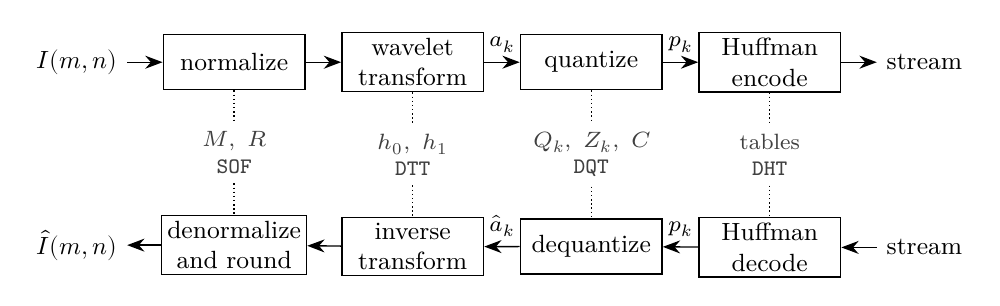
\begin{tikzpicture}[node distance=5mm and 4.5mm,
    stage/.style={box,minimum width=18mm,font=\small,align=center},
    side/.style={font=\footnotesize,align=center,text=black!75}]
  % encoder
  \node[font=\small] (img) {$I(m,n)$};
  \node[stage,right=of img] (norm) {normalize};
  \node[stage,right=of norm] (swt) {wavelet\\transform};
  \node[stage,right=of swt] (quant) {quantize};
  \node[stage,right=of quant] (huff) {Huffman\\encode};
  \node[font=\small,right=of huff] (out) {stream};
  \draw[->] (img) -- (norm);
  \draw[->] (norm) -- (swt);
  \draw[->] (swt) -- node[above,font=\footnotesize] {$a_k$} (quant);
  \draw[->] (quant) -- node[above,font=\footnotesize] {$p_k$} (huff);
  \draw[->] (huff) -- (out);
  % side information
  \node[side,below=4mm of norm] (sM) {$M,\ R$\\\marker{SOF}};
  \node[side,below=4mm of swt] (sF) {$h_0,\ h_1$\\\marker{DTT}};
  \node[side,below=4mm of quant] (sQ) {$Q_k,\ Z_k,\ C$\\\marker{DQT}};
  \node[side,below=4mm of huff] (sH) {tables\\\marker{DHT}};
  \foreach \s/\t in {sM/norm,sF/swt,sQ/quant,sH/huff} \draw[densely dotted] (\t) -- (\s);
  % decoder
  \node[stage,below=4mm of sM] (dnorm) {denormalize\\and round};
  \node[stage,below=4mm of sF] (dswt) {inverse\\transform};
  \node[stage,below=4mm of sQ] (dquant) {dequantize};
  \node[stage,below=4mm of sH] (dhuff) {Huffman\\decode};
  \node[font=\small] at (out |- dhuff) (in) {stream};
  \node[font=\small] at (img |- dnorm) (rec) {$\hat I(m,n)$};
  \foreach \s/\t in {sM/dnorm,sF/dswt,sQ/dquant,sH/dhuff} \draw[densely dotted] (\s) -- (\t);
  \draw[->] (in) -- (dhuff);
  \draw[->] (dhuff) -- node[above,font=\footnotesize] {$p_k$} (dquant);
  \draw[->] (dquant) -- node[above,font=\footnotesize] {$\hat a_k$} (dswt);
  \draw[->] (dswt) -- (dnorm);
  \draw[->] (dnorm) -- (rec);
\end{tikzpicture}

  \caption{The WSQ encoder (top) and decoder (bottom). The labels between the rows are the
  parameters the encoder writes into the stream and the marker segments that carry them.}
  \label{fig:pipeline}
\end{figure}

\subsection{Notation}

An image has $Y$ lines (rows) and $X$ samples per line (columns), the names the
specification uses in the frame header. A pixel is $I(m,n)$ with row $m$ and column $n$,
both counted from zero at the upper left corner. The 64 subbands are numbered
$k = 0,\dots,63$; subband $k$ has $X_k$ columns and $Y_k$ rows and holds the wavelet
coefficients $a_k(m,n)$. Quantization maps them to integer indices $p_k(m,n)$ with bin width
$Q_k$ and zero-bin width $Z_k$. The analysis filters are $h_0$ (lowpass) and $h_1$
(highpass); the synthesis filters are $f_0$ and $f_1$. For a real $x$, $\floor{x}$ is the
largest integer not above $x$ and $\ceil{x}$ the smallest integer not below it. Hexadecimal
byte values are written \hex{FF}.

\section{Normalization}
\label{sec:normalization}

Before the transform, the encoder maps the 8-bit samples to a signed range centred on zero
(Annex A.1 of the specification):
\begin{equation}
  I'(m,n) = \frac{I(m,n) - M}{R}.
  \label{eq:normalize}
\end{equation}
The specification leaves $M$ and $R$ to the encoder. Encoder number two uses the image mean
and the largest excursion from it, scaled to 128:
\begin{equation}
  M = \frac{1}{XY}\sum_{m,n} I(m,n), \qquad
  R = \frac{1}{128}\max\bigl(I_{\max} - M,\; M - I_{\min}\bigr),
  \label{eq:MR}
\end{equation}
so that $I'$ lies in $[-128, 128]$ whatever the contrast of the original. This makes the
subband variances, and with them the quantizer design of Section~\ref{sec:quantization},
independent of the image's brightness and contrast.

The decoder inverts the mapping and rounds to the nearest integer in the 8-bit range:
\begin{equation}
  \hat I(m,n) = \min\Bigl(255,\ \max\bigl(0,\ \floor{\hat I'(m,n)\,R + M + \tfrac12}\bigr)\Bigr).
  \label{eq:denormalize}
\end{equation}
The specification does not spell out the rounding; this is what the NIST reference decoder
does, and the compliance tolerance of one grey level (Section~\ref{sec:compliance}) absorbs
any other reasonable choice.

Two details are easy to miss. First, $M$ and $R$ travel in the frame header as decimal
\emph{scaled integers} (Section~\ref{sec:scaled}), which keep about five significant digits.
The encoder normalizes with the exact values and the decoder denormalizes with the rounded
ones; the mismatch is a relative error below $10^{-4}$ and has no visible effect. Second,
a constant image has $R = 0$, and Equation~\eqref{eq:normalize} divides by zero. The
specification does not cover this case, and an implementation has to decide what to do
(Section~\ref{sec:implementation}).

\section{The symmetric wavelet transform}
\label{sec:transform}

The transform is where WSQ gets its compression power. It does not reduce the amount of data
(it maps $XY$ samples to $XY$ coefficients) but it concentrates the image's energy: after the
transform, most coefficients are close to zero and the few large ones describe the ridge
pattern. This section builds the transform in four steps: a two-channel filter bank in one
dimension, the symmetric extension that makes it work on finite signals, the separable
two-dimensional version, and the particular cascade of 64 subbands the standard prescribes.

\subsection{The two-channel filter bank}

Figure~\ref{fig:filterbank} shows the building block (Annex A.2.1 of the specification). The
input $x$ goes through a lowpass filter $h_0$ and a highpass filter $h_1$, and each output is
\emph{decimated}: only every other sample is kept. The two half-length signals $a_0$ and $a_1$
are the \emph{subbands}. To reconstruct, each subband is \emph{upsampled} (a zero is inserted
between consecutive samples), filtered by a synthesis filter $f_0$ or $f_1$, and the two results
are added. With
\begin{equation*}
  (x * h)(k) = \sum_{n} x(n)\,h(k-n), \qquad
  ({\downarrow} y)(k) = y(2k), \qquad
  ({\uparrow} a)(n) = \begin{cases} a(n/2) & n \text{ even},\\ 0 & n \text{ odd},\end{cases}
\end{equation*}
the analysis bank computes $a_i = {\downarrow}(x * h_i)$ and the synthesis bank
$\hat x = f_0 * ({\uparrow} a_0) + f_1 * ({\uparrow} a_1)$.

\begin{figure}[ht]
  \centering
  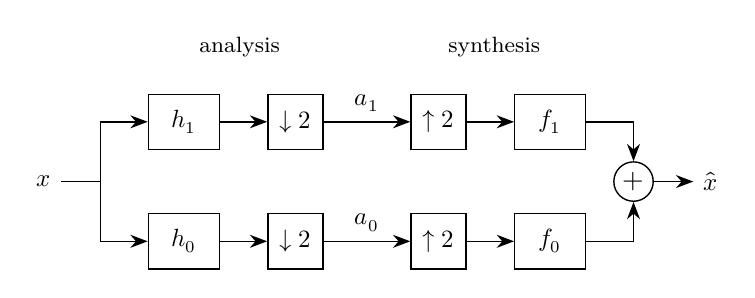
\begin{tikzpicture}[node distance=4mm and 6mm,
    f/.style={box,minimum width=9mm,font=\small},
    s/.style={box,minimum width=7mm,font=\small}]
  \node[font=\small] (x) {$x$};
  \coordinate[right=5mm of x] (fork);
  \node[f,above right=4mm and 6mm of fork] (h1) {$h_1$};
  \node[f,below right=4mm and 6mm of fork] (h0) {$h_0$};
  \node[s,right=of h1] (d1) {$\downarrow 2$};
  \node[s,right=of h0] (d0) {$\downarrow 2$};
  \node[s,right=11mm of d1] (u1) {$\uparrow 2$};
  \node[s,right=11mm of d0] (u0) {$\uparrow 2$};
  \node[f,right=of u1] (f1) {$f_1$};
  \node[f,right=of u0] (f0) {$f_0$};
  \node[op,right=8mm of $(f1)!0.5!(f0)$] (sum) {$+$};
  \node[font=\small,right=5mm of sum] (xh) {$\hat x$};
  \draw (x) -- (fork);
  \draw[->] (fork) |- (h1);
  \draw[->] (fork) |- (h0);
  \draw[->] (h1) -- (d1);
  \draw[->] (h0) -- (d0);
  \draw[->] (d1) -- node[above,font=\small] {$a_1$} (u1);
  \draw[->] (d0) -- node[above,font=\small] {$a_0$} (u0);
  \draw[->] (u1) -- (f1);
  \draw[->] (u0) -- (f0);
  \draw[->] (f1) -| (sum);
  \draw[->] (f0) -| (sum);
  \draw[->] (sum) -- (xh);
  \node[font=\footnotesize,above=7mm of $(h1)!0.5!(d1)$] {analysis};
  \node[font=\footnotesize,above=7mm of $(u1)!0.5!(f1)$] {synthesis};
\end{tikzpicture}

  \caption{Two-channel subband coder. With the right filters the output equals the input.}
  \label{fig:filterbank}
\end{figure}

Decimation discards half the samples of each branch, so each subband on its own is aliased.
The synthesis filters are chosen so that the aliasing of the two branches cancels and
$\hat x = x$ exactly (\emph{perfect reconstruction}). WSQ uses the \emph{anti-aliasing
relations}
\begin{equation}
  f_0(n) = (-1)^n\, h_1(n-1), \qquad f_1(n) = (-1)^{n-1}\, h_0(n-1),
  \label{eq:antialias}
\end{equation}
which make the aliasing terms cancel identically. Together with a biorthogonality condition
between $h_0$ and $h_1$ they give perfect reconstruction. Because of
Equation~\eqref{eq:antialias}, a WSQ file only carries the analysis filters, and only half of
each, since they are symmetric.

\subsection{Linear-phase filters}

WSQ allows two families of symmetric (linear-phase) filter banks (Annex A.2.1.1).
\begin{description}[leftmargin=0pt]
  \item[Whole-sample symmetric (WS) banks] have odd-length filters. The lowpass filter $h_0$
    is symmetric about $0$, $h_0(-n) = h_0(n)$, and runs from $-r_0$ to $r_0$ (length
    $L_0 = 2r_0+1$). The highpass filter $h_1$ is symmetric about $-1$,
    $h_1(-1-n) = h_1(n-1)$, and runs from $-1-r_1$ to $-1+r_1$ (length $L_1 = 2r_1+1$).
    The file carries $h_0(0),\dots,h_0(r_0)$ and $h_1(-1),\dots,h_1(r_1-1)$.
  \item[Half-sample symmetric (HS) banks] have even-length filters, both centred at
    $-\tfrac12$ and running from $-r_i$ to $r_i - 1$ (length $L_i = 2r_i$). The lowpass
    filter is symmetric, $h_0(-1-n) = h_0(n)$, and the highpass filter antisymmetric,
    $h_1(-1-n) = -h_1(n)$. The file carries $h_i(0),\dots,h_i(r_i-1)$.
\end{description}
Decoders must accept lengths up to 31 (WS) and 32 (HS). Encoder number two uses the WS bank
of Table~\ref{tab:filters}, a 9-tap lowpass and a 7-tap highpass filter from the family of
Cohen, Daubechies and Feauveau that Antonini et al.\ introduced for image coding
\cite{antonini1992}; JPEG~2000 later adopted the same pair. The specification also gives
their exact values: with
\begin{equation*}
  A = \Bigl(\frac{-14\sqrt{15}+63}{1080\sqrt{15}}\Bigr)^{1/3},\quad
  B = \Bigl(\frac{-14\sqrt{15}-63}{1080\sqrt{15}}\Bigr)^{1/3},\quad
  x_1 = A + B - \tfrac16,\quad
  x_2 = -\tfrac{A+B}{2} - \tfrac16 + \mathrm{i}\,\tfrac{\sqrt3}{2}(A-B),
\end{equation*}
(real cube roots), the taps are
\begin{align*}
  h_0(0)     &= -5\sqrt2\,x_1\,(48|x_2|^2 - 16\,\mathrm{Re}\,x_2 + 3)/32, &
  h_1(-1)    &= \sqrt2\,(6x_1-1)/(16x_1),\\
  h_0(\pm1)  &= -5\sqrt2\,x_1\,(8|x_2|^2 - \mathrm{Re}\,x_2)/8, &
  h_1(-2) = h_1(0) &= -\sqrt2\,(16x_1-1)/(64x_1),\\
  h_0(\pm2)  &= -5\sqrt2\,x_1\,(4|x_2|^2 + 4\,\mathrm{Re}\,x_2 - 1)/16, &
  h_1(-3) = h_1(1) &= \sqrt2\,(2x_1+1)/(32x_1),\\
  h_0(\pm3)  &= -5\sqrt2\,x_1\,\mathrm{Re}\,x_2/8, &
  h_1(-4) = h_1(2) &= -\sqrt2/(64x_1),\\
  h_0(\pm4)  &= -5\sqrt2\,x_1/64.
\end{align*}
The lowpass taps add up to $\sqrt2$ and the highpass taps to zero.

\begin{table}[ht]
  \centering\small
  \begin{tabular}{@{}lr@{\qquad}lr@{}}
    \toprule
    tap & value & tap & value \\
    \midrule
    $h_0(0)$       &  0.852698679009403 & $h_1(-1)$       &  0.788485616405664 \\
    $h_0(\pm1)$    &  0.377402855612654 & $h_1(-2),h_1(0)$ & $-0.418092273222212$ \\
    $h_0(\pm2)$    & $-0.110624404418423$ & $h_1(-3),h_1(1)$ & $-0.040689417609558$ \\
    $h_0(\pm3)$    & $-0.023849465019380$ & $h_1(-4),h_1(2)$ &  0.064538882628938 \\
    $h_0(\pm4)$    &  0.037828455506995 & & \\
    \bottomrule
  \end{tabular}
  \caption{The analysis filters of encoder number two (Part 3, Table 1).}
  \label{tab:filters}
\end{table}

\subsection{Finite signals: symmetric extension}
\label{sec:extension}

A filter bank is defined on infinite signals, while an image row has $N_0$ samples. Treating
the samples outside the row as zero, or wrapping the row around periodically, creates a jump
at the borders. A jump has energy at every frequency, so it would fill the highpass subbands
with large coefficients that carry no information about the fingerprint.

WSQ mirrors the signal at its ends instead (Annex A.2.2), as in Figure~\ref{fig:extension}.
With a WS bank the row is reflected about its first and last samples without repeating them,
which gives a signal of period $2N_0-2$; with an HS bank it is reflected about the half-sample
points $-\tfrac12$ and $N_0-\tfrac12$, repeating the end samples, which gives period $2N_0$.
The mirrored signal is continuous at the borders. Moreover, a symmetric signal filtered by a
symmetric filter is again symmetric, so the subbands of the extended signal are themselves
symmetric and periodic, and only a non-redundant part of each needs to be stored. That part has
$\ceil{N_0/2}$ samples for the lowpass subband and $\floor{N_0/2}$ for the highpass one:
$N_0$ samples in, $N_0$ coefficients out. The specification calls this the \emph{symmetric
wavelet transform} (SWT) \cite{brislawn1992}.

\begin{figure}[ht]
  \centering
  % Generated by tools/gen_figures.py; do not edit by hand.
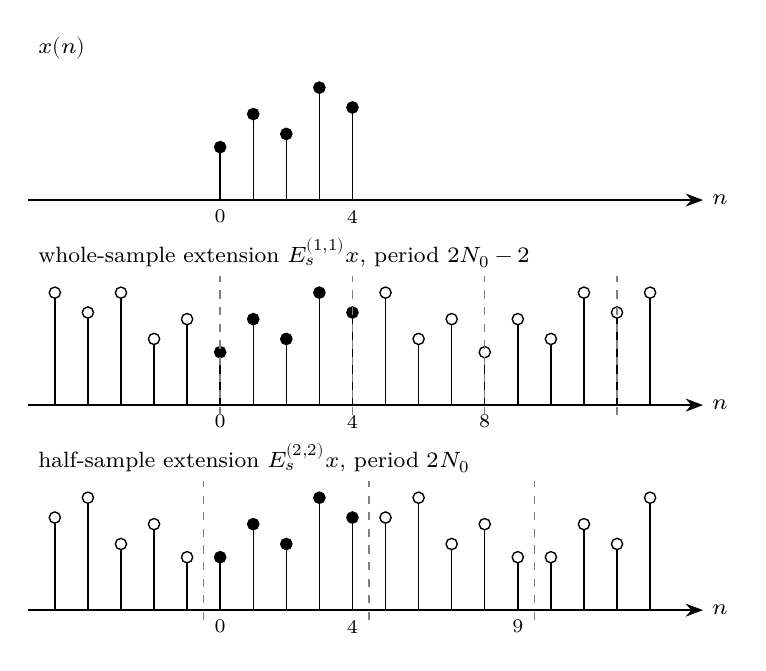
\begin{tikzpicture}[x=0.42cm,y=0.42cm]
  \draw[->] (-5.8,-0.0) -- (14.6,-0.0) node[right,font=\footnotesize] {$n$};
  \node[anchor=west,font=\footnotesize] at (-5.8,4.6) {$x(n)$};
  \draw (0,-0.0) -- (0,1.6);
  \fill[black,draw=black] (0,1.6) circle (0.17);
  \draw (1,-0.0) -- (1,2.6);
  \fill[black,draw=black] (1,2.6) circle (0.17);
  \draw (2,-0.0) -- (2,2.0);
  \fill[black,draw=black] (2,2.0) circle (0.17);
  \draw (3,-0.0) -- (3,3.4);
  \fill[black,draw=black] (3,3.4) circle (0.17);
  \draw (4,-0.0) -- (4,2.8);
  \fill[black,draw=black] (4,2.8) circle (0.17);
  \node[below,font=\scriptsize] at (0,-0.0) {0};
  \node[below,font=\scriptsize] at (4,-0.0) {4};
  \draw[->] (-5.8,-6.2) -- (14.6,-6.2) node[right,font=\footnotesize] {$n$};
  \node[anchor=west,font=\footnotesize] at (-5.8,-1.6000000000000005) {whole-sample extension $E_s^{(1,1)}x$, period $2N_0-2$};
  \draw (-5,-6.2) -- (-5,-2.8000000000000003);
  \fill[white,draw=black] (-5,-2.8000000000000003) circle (0.17);
  \draw (-4,-6.2) -- (-4,-3.4000000000000004);
  \fill[white,draw=black] (-4,-3.4000000000000004) circle (0.17);
  \draw (-3,-6.2) -- (-3,-2.8000000000000003);
  \fill[white,draw=black] (-3,-2.8000000000000003) circle (0.17);
  \draw (-2,-6.2) -- (-2,-4.2);
  \fill[white,draw=black] (-2,-4.2) circle (0.17);
  \draw (-1,-6.2) -- (-1,-3.6);
  \fill[white,draw=black] (-1,-3.6) circle (0.17);
  \draw (0,-6.2) -- (0,-4.6);
  \fill[black,draw=black] (0,-4.6) circle (0.17);
  \draw (1,-6.2) -- (1,-3.6);
  \fill[black,draw=black] (1,-3.6) circle (0.17);
  \draw (2,-6.2) -- (2,-4.2);
  \fill[black,draw=black] (2,-4.2) circle (0.17);
  \draw (3,-6.2) -- (3,-2.8000000000000003);
  \fill[black,draw=black] (3,-2.8000000000000003) circle (0.17);
  \draw (4,-6.2) -- (4,-3.4000000000000004);
  \fill[black,draw=black] (4,-3.4000000000000004) circle (0.17);
  \draw (5,-6.2) -- (5,-2.8000000000000003);
  \fill[white,draw=black] (5,-2.8000000000000003) circle (0.17);
  \draw (6,-6.2) -- (6,-4.2);
  \fill[white,draw=black] (6,-4.2) circle (0.17);
  \draw (7,-6.2) -- (7,-3.6);
  \fill[white,draw=black] (7,-3.6) circle (0.17);
  \draw (8,-6.2) -- (8,-4.6);
  \fill[white,draw=black] (8,-4.6) circle (0.17);
  \draw (9,-6.2) -- (9,-3.6);
  \fill[white,draw=black] (9,-3.6) circle (0.17);
  \draw (10,-6.2) -- (10,-4.2);
  \fill[white,draw=black] (10,-4.2) circle (0.17);
  \draw (11,-6.2) -- (11,-2.8000000000000003);
  \fill[white,draw=black] (11,-2.8000000000000003) circle (0.17);
  \draw (12,-6.2) -- (12,-3.4000000000000004);
  \fill[white,draw=black] (12,-3.4000000000000004) circle (0.17);
  \draw (13,-6.2) -- (13,-2.8000000000000003);
  \fill[white,draw=black] (13,-2.8000000000000003) circle (0.17);
  \node[below,font=\scriptsize] at (0,-6.2) {0};
  \node[below,font=\scriptsize] at (4,-6.2) {4};
  \node[below,font=\scriptsize] at (8,-6.2) {8};
  \draw[dashed,gray] (0,-6.5) -- (0,-2.3000000000000003);
  \draw[dashed,gray] (4,-6.5) -- (4,-2.3000000000000003);
  \draw[dashed,gray] (8,-6.5) -- (8,-2.3000000000000003);
  \draw[dashed,gray] (12,-6.5) -- (12,-2.3000000000000003);
  \draw[->] (-5.8,-12.4) -- (14.6,-12.4) node[right,font=\footnotesize] {$n$};
  \node[anchor=west,font=\footnotesize] at (-5.8,-7.800000000000001) {half-sample extension $E_s^{(2,2)}x$, period $2N_0$};
  \draw (-5,-12.4) -- (-5,-9.600000000000001);
  \fill[white,draw=black] (-5,-9.600000000000001) circle (0.17);
  \draw (-4,-12.4) -- (-4,-9.0);
  \fill[white,draw=black] (-4,-9.0) circle (0.17);
  \draw (-3,-12.4) -- (-3,-10.4);
  \fill[white,draw=black] (-3,-10.4) circle (0.17);
  \draw (-2,-12.4) -- (-2,-9.8);
  \fill[white,draw=black] (-2,-9.8) circle (0.17);
  \draw (-1,-12.4) -- (-1,-10.8);
  \fill[white,draw=black] (-1,-10.8) circle (0.17);
  \draw (0,-12.4) -- (0,-10.8);
  \fill[black,draw=black] (0,-10.8) circle (0.17);
  \draw (1,-12.4) -- (1,-9.8);
  \fill[black,draw=black] (1,-9.8) circle (0.17);
  \draw (2,-12.4) -- (2,-10.4);
  \fill[black,draw=black] (2,-10.4) circle (0.17);
  \draw (3,-12.4) -- (3,-9.0);
  \fill[black,draw=black] (3,-9.0) circle (0.17);
  \draw (4,-12.4) -- (4,-9.600000000000001);
  \fill[black,draw=black] (4,-9.600000000000001) circle (0.17);
  \draw (5,-12.4) -- (5,-9.600000000000001);
  \fill[white,draw=black] (5,-9.600000000000001) circle (0.17);
  \draw (6,-12.4) -- (6,-9.0);
  \fill[white,draw=black] (6,-9.0) circle (0.17);
  \draw (7,-12.4) -- (7,-10.4);
  \fill[white,draw=black] (7,-10.4) circle (0.17);
  \draw (8,-12.4) -- (8,-9.8);
  \fill[white,draw=black] (8,-9.8) circle (0.17);
  \draw (9,-12.4) -- (9,-10.8);
  \fill[white,draw=black] (9,-10.8) circle (0.17);
  \draw (10,-12.4) -- (10,-10.8);
  \fill[white,draw=black] (10,-10.8) circle (0.17);
  \draw (11,-12.4) -- (11,-9.8);
  \fill[white,draw=black] (11,-9.8) circle (0.17);
  \draw (12,-12.4) -- (12,-10.4);
  \fill[white,draw=black] (12,-10.4) circle (0.17);
  \draw (13,-12.4) -- (13,-9.0);
  \fill[white,draw=black] (13,-9.0) circle (0.17);
  \node[below,font=\scriptsize] at (0,-12.4) {0};
  \node[below,font=\scriptsize] at (4,-12.4) {4};
  \node[below,font=\scriptsize] at (9,-12.4) {9};
  \draw[dashed,gray] (-0.5,-12.700000000000001) -- (-0.5,-8.5);
  \draw[dashed,gray] (4.5,-12.700000000000001) -- (4.5,-8.5);
  \draw[dashed,gray] (9.5,-12.700000000000001) -- (9.5,-8.5);
\end{tikzpicture}

  \caption{A signal of $N_0 = 5$ samples (filled) and its two symmetric extensions (hollow
  samples are mirror images). Dashed lines mark the centres of symmetry.}
  \label{fig:extension}
\end{figure}

In formulas, let $\tilde x$ be the extended signal. For a WS bank, with period $P = 2N_0-2$
and $u = n \bmod P$ taken in $[0, P)$,
\begin{equation}
  \tilde x(n) = x\bigl(u\bigr) \text{ if } u < N_0, \qquad \tilde x(n) = x\bigl(P-u\bigr) \text{ otherwise};
  \label{eq:wsext}
\end{equation}
for an HS bank, with $P = 2N_0$, the second case reads $x(P-1-u)$. (A one-sample signal
extends to a constant.) The subbands are
\begin{equation}
  a_0(k) = \sum_j h_0(j)\,\tilde x(2k-j), \quad 0 \le k < \ceil{N_0/2}, \qquad
  a_1(k) = \sum_j h_1(j)\,\tilde x(2k-j), \quad 0 \le k < \floor{N_0/2}.
  \label{eq:analysis}
\end{equation}
With the WS bank of Table~\ref{tab:filters}, $a_0(k)$ is a weighted average centred on the
even sample $2k$, and $a_1(k)$ a difference centred on the odd sample $2k+1$ (because $h_1$ is
centred at $-1$). Algorithm~\ref{alg:analysis} spells this out.

\begin{algorithm}[ht]
  \caption{One-dimensional symmetric wavelet analysis.}
  \label{alg:analysis}
  \begin{algorithmic}[1]
    \Require $x(0),\dots,x(N_0-1)$; analysis filters $h_0, h_1$; bank type WS or HS
    \Ensure $a_0$ with $\ceil{N_0/2}$ values, $a_1$ with $\floor{N_0/2}$ values
    \Function{Ext}{$n$} \Comment{index into $x$ of sample $n$ of the extension}
      \If{$N_0 = 1$} \Return $0$ \EndIf
      \If{WS} \State $P \gets 2N_0 - 2$;\ $u \gets n \bmod P$;\ \Return $u$ \textbf{if} $u < N_0$ \textbf{else} $P - u$
      \Else \State $P \gets 2N_0$;\ $u \gets n \bmod P$;\ \Return $u$ \textbf{if} $u < N_0$ \textbf{else} $P - 1 - u$
      \EndIf
    \EndFunction
    \For{$k \gets 0$ \textbf{to} $\ceil{N_0/2}-1$}
      \State $a_0(k) \gets \sum_{j} h_0(j)\; x\bigl(\Call{Ext}{2k - j}\bigr)$ \Comment{$j$ over the taps of $h_0$}
    \EndFor
    \For{$k \gets 0$ \textbf{to} $\floor{N_0/2}-1$}
      \State $a_1(k) \gets \sum_{j} h_1(j)\; x\bigl(\Call{Ext}{2k - j}\bigr)$
    \EndFor
  \end{algorithmic}
\end{algorithm}

\subsection{Synthesis}

To invert, the decoder rebuilds the full periodic subbands $b_0$ and $b_1$ from the stored
halves using their symmetries (Annex A.2.2.1 and its Table A.1), then applies the synthesis
bank. The symmetries follow from those of the extension and the filters, and they lead to
simple index maps. Let $\rho_0 = \ceil{N_0/2}$ and $\rho_1 = \floor{N_0/2}$ be the stored
lengths.
\begin{itemize}
  \item WS bank: both subbands have period $P = N_0 - 1$. With $u = k \bmod P$,
    \[
      b_0(k) = a_0\bigl(\min(u,\,P-u)\bigr), \qquad b_1(k) = a_1\bigl(\min(u,\,P-1-u)\bigr).
    \]
    The lowpass subband is symmetric about $0$ and the highpass one about $-\tfrac12$.
  \item HS bank: both subbands have period $N_0$. With $u = k \bmod N_0$ and $v = N_0-1-u$,
    \[
      b_0(k) = a_0\bigl(\min(u,v)\bigr), \qquad
      b_1(k) = \begin{cases} a_1(u) & u < v,\\ -a_1(v) & u > v,\\ 0 & u = v. \end{cases}
    \]
    The highpass subband is antisymmetric, and when $N_0$ is odd its centre sample is zero,
    which is why only $(N_0-1)/2$ values are stored.
\end{itemize}
The reconstruction is then
\begin{equation}
  x(n) = \sum_{k} f_0(n-2k)\,b_0(k) + \sum_{k} f_1(n-2k)\,b_1(k), \qquad 0 \le n < N_0,
  \label{eq:synthesis}
\end{equation}
where the sums run over the $k$ for which the filter tap exists. Algorithm~\ref{alg:synthesis}
writes it out. These index maps are equivalent to the extension operators of the
specification; implemented as written, Algorithms~\ref{alg:analysis} and~\ref{alg:synthesis}
reconstruct random signals of every length from 1 to 101 to within $10^{-13}$, with the
encoder number two filters and with the Haar HS bank.

\begin{algorithm}[ht]
  \caption{One-dimensional symmetric wavelet synthesis.}
  \label{alg:synthesis}
  \begin{algorithmic}[1]
    \Require $a_0$ ($\rho_0$ values), $a_1$ ($\rho_1$ values); synthesis filters $f_0, f_1$ from Eq.~\eqref{eq:antialias}
    \Ensure $x(0),\dots,x(N_0-1)$, with $N_0 = \rho_0 + \rho_1$
    \Function{B$_0$}{$k$}
      \If{WS} \If{$N_0 = 1$} \Return $a_0(0)$ \EndIf
        \State $P \gets N_0 - 1$;\ $u \gets k \bmod P$;\ \Return $a_0(\min(u, P-u))$
      \Else \State $u \gets k \bmod N_0$;\ \Return $a_0(\min(u, N_0-1-u))$
      \EndIf
    \EndFunction
    \Function{B$_1$}{$k$}
      \If{WS} \State $P \gets N_0 - 1$;\ $u \gets k \bmod P$;\ \Return $a_1(\min(u, P-1-u))$
      \Else \State $u \gets k \bmod N_0$;\ $v \gets N_0-1-u$
        \If{$u < v$} \Return $a_1(u)$ \ElsIf{$u > v$} \Return $-a_1(v)$ \Else\ \Return $0$ \EndIf
      \EndIf
    \EndFunction
    \For{$n \gets 0$ \textbf{to} $N_0-1$}
      \State $x(n) \gets \sum_{t:\ n-t \text{ even}} f_0(t)\,\Call{B$_0$}{(n-t)/2}$
      \State $x(n) \gets x(n) + \sum_{t:\ n-t \text{ even}} f_1(t)\,\Call{B$_1$}{(n-t)/2}$ \Comment{skipped when $\rho_1 = 0$}
    \EndFor
  \end{algorithmic}
\end{algorithm}

\subsection{Two dimensions}

Images are transformed separably (Annex A.2.3): every row is passed through the
one-dimensional SWT, and then every column of the result. The rows yield a lowpass half on
the left and a highpass half on the right; the columns split each half again into a top and a
bottom part. One level therefore produces four subbands (Figure~\ref{fig:twodim}). The
specification names them $a_{ij}$, where $i$ is the filter applied along the rows (horizontal
direction) and $j$ the one applied along the columns: $a_{10}$ is highpass horizontally and
lowpass vertically, so it responds to vertical edges. The inverse transform does the opposite,
columns first and rows second.

\begin{figure}[ht]
  \centering
  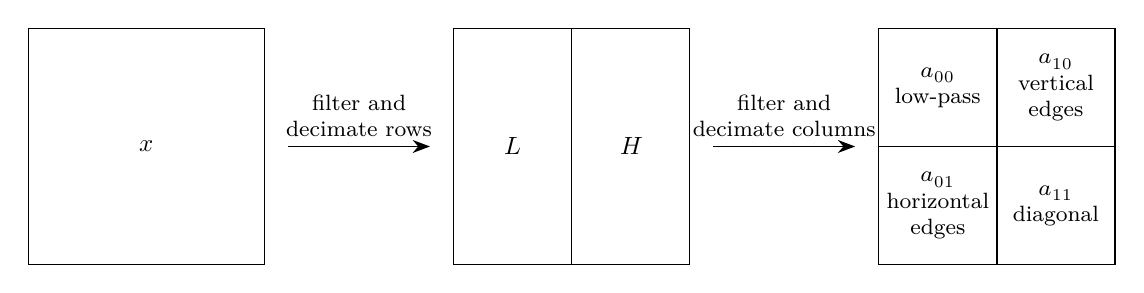
\begin{tikzpicture}[x=1cm,y=-1cm,font=\small]
  % input
  \draw (0,0) rectangle (3,3);
  \node at (1.5,1.5) {$x$};
  \draw[->] (3.3,1.5) -- node[above,font=\footnotesize,align=center] {filter and\\decimate rows} (5.1,1.5);
  % after rows
  \draw (5.4,0) rectangle (8.4,3);
  \draw (6.9,0) -- (6.9,3);
  \node at (6.15,1.5) {$L$};
  \node at (7.65,1.5) {$H$};
  \draw[->] (8.7,1.5) -- node[above,font=\footnotesize,align=center] {filter and\\decimate columns} (10.5,1.5);
  % after columns
  \draw (10.8,0) rectangle (13.8,3);
  \draw (12.3,0) -- (12.3,3) (10.8,1.5) -- (13.8,1.5);
  \node[align=center,font=\footnotesize] at (11.55,0.75) {$a_{00}$\\low-pass};
  \node[align=center,font=\footnotesize] at (13.05,0.75) {$a_{10}$\\vertical\\edges};
  \node[align=center,font=\footnotesize] at (11.55,2.25) {$a_{01}$\\horizontal\\edges};
  \node[align=center,font=\footnotesize] at (13.05,2.25) {$a_{11}$\\diagonal};
\end{tikzpicture}

  \caption{One level of the separable two-dimensional transform.}
  \label{fig:twodim}
\end{figure}

\subsection{Spectral inversion}
\label{sec:inversion}

WSQ applies the filter bank again to some of the subbands it produces. Splitting the lowpass
subband again is straightforward, but splitting a highpass subband involves a subtlety. A
cosine of frequency $\omega$ sampled at the even positions becomes
$\cos(2\omega k) = \cos\bigl((2\pi - 2\omega)k\bigr)$, so decimation maps the band
$[\pi/2, \pi]$ onto $[0, \pi]$ \emph{in reverse}: the highest frequencies of the original end up
at the lowest frequencies of the subband. The highpass subband is spectrally mirrored.
If it is split again, its lowpass half holds the original frequencies near $\pi$, and its
highpass half those near $\pi/2$.

The specification orders subbands by the original frequency they represent, from the top left
(lowest) to the bottom right (highest). A mirrored region must therefore store the highpass
output of its split \emph{first}. Figure~\ref{fig:inversion} shows two levels in one
dimension: the four bands, in increasing frequency, have filter paths $00$, $01$, $11$ and $10$,
a Gray code. In general, a band's position along an axis is obtained from its filter path
(0 for lowpass, 1 for highpass) by a running exclusive-or, and the
\emph{Filter Bank Path} table of Figure A.5 of the specification follows this rule.

\begin{figure}[ht]
  \centering
  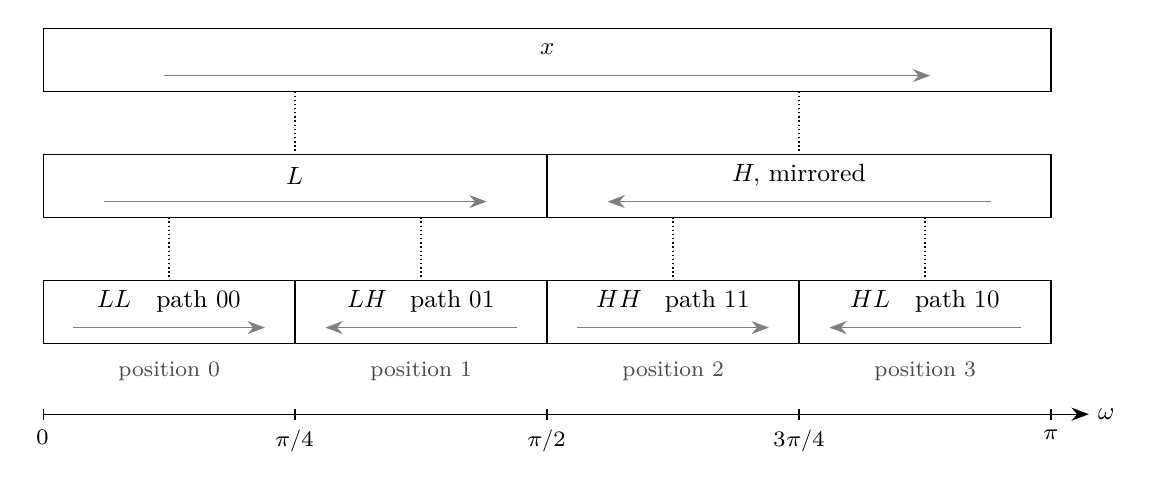
\begin{tikzpicture}[x=3.2cm,y=-1cm,font=\small]
  % a band from #1 to #2 on row #3, label #4, spectrum orientation #5 (1 normal, -1 mirrored)
  \newcommand{\band}[5]{%
    \draw (#1,#3) rectangle (#2,#3+0.8);
    \node at ({(#1+#2)/2},#3+0.27) {#4};
    \ifnum#5=1
      \draw[->,gray] ({#1+0.12*(#2-#1)},#3+0.6) -- ({#2-0.12*(#2-#1)},#3+0.6);
    \else
      \draw[<-,gray] ({#1+0.12*(#2-#1)},#3+0.6) -- ({#2-0.12*(#2-#1)},#3+0.6);
    \fi}
  \band{0}{4}{0}{$x$}{1}
  \band{0}{2}{1.6}{$L$}{1}
  \band{2}{4}{1.6}{$H$, mirrored}{-1}
  \band{0}{1}{3.2}{$LL$\quad path $00$}{1}
  \band{1}{2}{3.2}{$LH$\quad path $01$}{-1}
  \band{2}{3}{3.2}{$HH$\quad path $11$}{1}
  \band{3}{4}{3.2}{$HL$\quad path $10$}{-1}
  \draw[densely dotted] (1,0.8) -- (1,1.6) (3,0.8) -- (3,1.6);
  \draw[densely dotted] (0.5,2.4) -- (0.5,3.2) (1.5,2.4) -- (1.5,3.2) (2.5,2.4) -- (2.5,3.2) (3.5,2.4) -- (3.5,3.2);
  \foreach \p in {0,1,2,3}
    \node[font=\footnotesize,text=black!70] at (\p+0.5,4.35) {position \p};
  \draw[->] (0,4.9) -- (4.15,4.9) node[right] {$\omega$};
  \foreach \t/\l in {0/{0},1/{\pi/4},2/{\pi/2},3/{3\pi/4},4/{\pi}}
    \draw (\t,4.83) -- (\t,4.97) node[below,font=\footnotesize] {$\l$};
\end{tikzpicture}

  \caption{Spectral inversion in two levels of a one-dimensional decomposition. Grey arrows
  show the orientation of each band's spectrum after decimation; a mirrored band places its
  highpass half first, so the four outputs end up ordered by frequency.}
  \label{fig:inversion}
\end{figure}

This gives a simple bookkeeping rule. Give every region two flags, $\iota_x$ and $\iota_y$,
meaning \emph{mirrored along the horizontal (vertical) axis}. The whole image has both flags
clear. When a region is split, the child placed second along an axis (on the right, or at the
bottom) is mirrored along that axis, and the child placed first is not, whatever the flags of
the parent. Inside a mirrored region, the highpass part comes first. Since the lowpass part
always has $\ceil{N/2}$ samples and the highpass part $\floor{N/2}$, splitting a mirrored
region of odd length $N$ puts the \emph{shorter} part first.

\subsection{The 64-subband decomposition}
\label{sec:subbands}

The specification fixes one decomposition for all images, shown in Figure~\ref{fig:subbands}
(Figure A.5 of the specification). It can be described in three steps.
\begin{enumerate}
  \item Two levels of splitting turn the image into a $4 \times 4$ grid of cells, each about
    a quarter of the image in each direction.
  \item The three cells with the lowest frequencies, at grid positions $(0,0)$, $(0,1)$ and
    $(1,0)$ (row, column), are each split two more times into $4 \times 4$ grids of their own.
  \item Inside the first of these, the cell at its own position $(0,0)$, the lowest-frequency
    band of the image, is split once more into four.
\end{enumerate}
Subbands are numbered by visiting the grids in \emph{Z-order} (top left, top right, bottom
left, bottom right, recursively), so that each refined cell is replaced by its own children in
Z-order. This gives subbands 0--3 (one thirty-second of the image along each axis), 4--50 (one
sixteenth) and 51--63 (one quarter). The downsampling factor $m_k$, the ratio of image area to
subband area, is $1024$, $256$ and $16$ in these three groups, and
$4/1024 + 47/256 + 13/16 = 1$.

\begin{figure}[ht]
  \centering
  % Generated by tools/gen_figures.py; do not edit by hand.
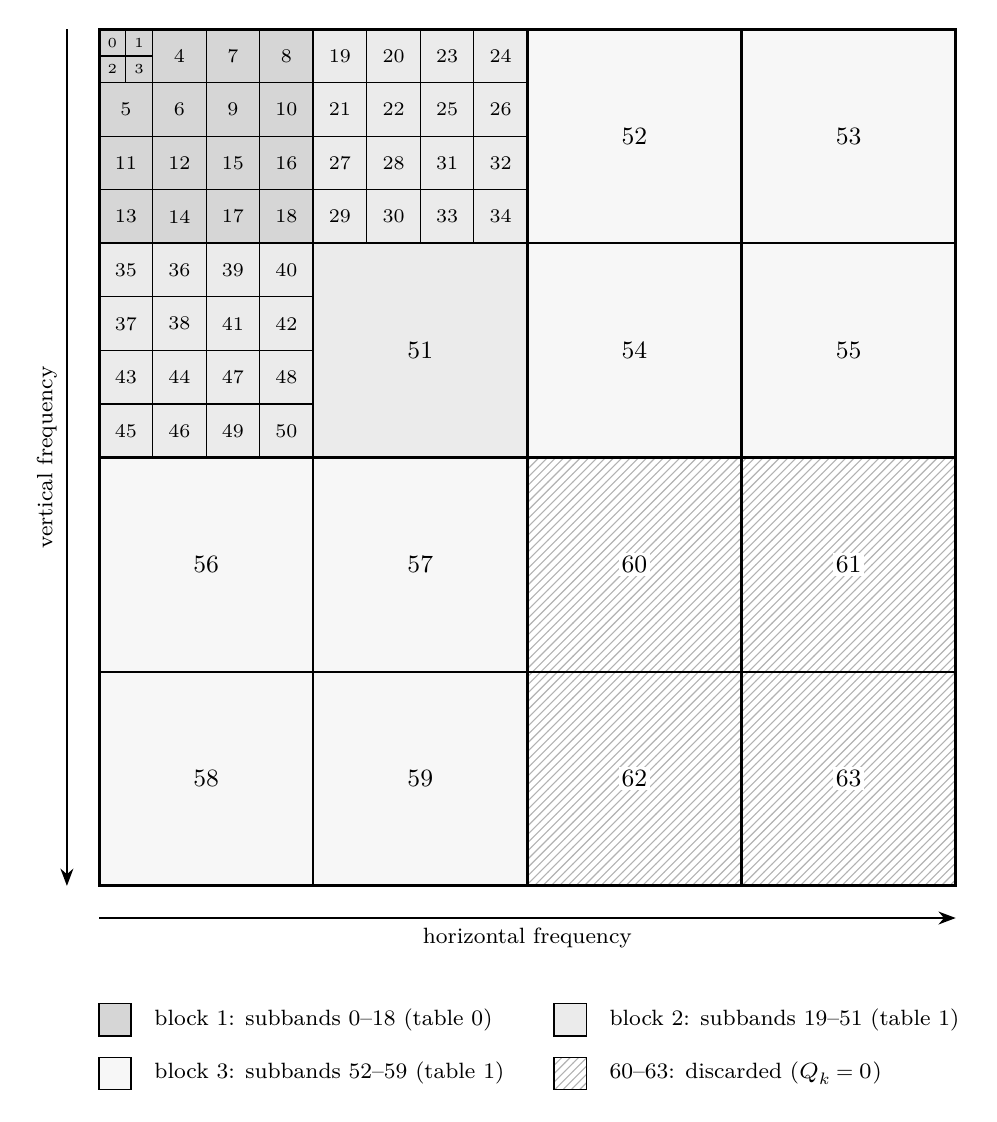
\begin{tikzpicture}[x=0.34cm,y=-0.34cm]
  \path[fill=gray!32] (0,0) rectangle (1,1);
  \path[fill=gray!32] (1,0) rectangle (2,1);
  \path[fill=gray!32] (0,1) rectangle (1,2);
  \path[fill=gray!32] (1,1) rectangle (2,2);
  \path[fill=gray!32] (2,0) rectangle (4,2);
  \path[fill=gray!32] (0,2) rectangle (2,4);
  \path[fill=gray!32] (2,2) rectangle (4,4);
  \path[fill=gray!32] (4,0) rectangle (6,2);
  \path[fill=gray!32] (6,0) rectangle (8,2);
  \path[fill=gray!32] (4,2) rectangle (6,4);
  \path[fill=gray!32] (6,2) rectangle (8,4);
  \path[fill=gray!32] (0,4) rectangle (2,6);
  \path[fill=gray!32] (2,4) rectangle (4,6);
  \path[fill=gray!32] (0,6) rectangle (2,8);
  \path[fill=gray!32] (2,6) rectangle (4,8);
  \path[fill=gray!32] (4,4) rectangle (6,6);
  \path[fill=gray!32] (6,4) rectangle (8,6);
  \path[fill=gray!32] (4,6) rectangle (6,8);
  \path[fill=gray!32] (6,6) rectangle (8,8);
  \path[fill=gray!16] (8,0) rectangle (10,2);
  \path[fill=gray!16] (10,0) rectangle (12,2);
  \path[fill=gray!16] (8,2) rectangle (10,4);
  \path[fill=gray!16] (10,2) rectangle (12,4);
  \path[fill=gray!16] (12,0) rectangle (14,2);
  \path[fill=gray!16] (14,0) rectangle (16,2);
  \path[fill=gray!16] (12,2) rectangle (14,4);
  \path[fill=gray!16] (14,2) rectangle (16,4);
  \path[fill=gray!16] (8,4) rectangle (10,6);
  \path[fill=gray!16] (10,4) rectangle (12,6);
  \path[fill=gray!16] (8,6) rectangle (10,8);
  \path[fill=gray!16] (10,6) rectangle (12,8);
  \path[fill=gray!16] (12,4) rectangle (14,6);
  \path[fill=gray!16] (14,4) rectangle (16,6);
  \path[fill=gray!16] (12,6) rectangle (14,8);
  \path[fill=gray!16] (14,6) rectangle (16,8);
  \path[fill=gray!16] (0,8) rectangle (2,10);
  \path[fill=gray!16] (2,8) rectangle (4,10);
  \path[fill=gray!16] (0,10) rectangle (2,12);
  \path[fill=gray!16] (2,10) rectangle (4,12);
  \path[fill=gray!16] (4,8) rectangle (6,10);
  \path[fill=gray!16] (6,8) rectangle (8,10);
  \path[fill=gray!16] (4,10) rectangle (6,12);
  \path[fill=gray!16] (6,10) rectangle (8,12);
  \path[fill=gray!16] (0,12) rectangle (2,14);
  \path[fill=gray!16] (2,12) rectangle (4,14);
  \path[fill=gray!16] (0,14) rectangle (2,16);
  \path[fill=gray!16] (2,14) rectangle (4,16);
  \path[fill=gray!16] (4,12) rectangle (6,14);
  \path[fill=gray!16] (6,12) rectangle (8,14);
  \path[fill=gray!16] (4,14) rectangle (6,16);
  \path[fill=gray!16] (6,14) rectangle (8,16);
  \path[fill=gray!16] (8,8) rectangle (16,16);
  \path[fill=gray!6] (16,0) rectangle (24,8);
  \path[fill=gray!6] (24,0) rectangle (32,8);
  \path[fill=gray!6] (16,8) rectangle (24,16);
  \path[fill=gray!6] (24,8) rectangle (32,16);
  \path[fill=gray!6] (0,16) rectangle (8,24);
  \path[fill=gray!6] (8,16) rectangle (16,24);
  \path[fill=gray!6] (0,24) rectangle (8,32);
  \path[fill=gray!6] (8,24) rectangle (16,32);
  \path[pattern=north east lines,pattern color=gray!60] (16,16) rectangle (24,24);
  \path[pattern=north east lines,pattern color=gray!60] (24,16) rectangle (32,24);
  \path[pattern=north east lines,pattern color=gray!60] (16,24) rectangle (24,32);
  \path[pattern=north east lines,pattern color=gray!60] (24,24) rectangle (32,32);
  \draw[line width=0.4pt] (0,0) rectangle (1,1);
  \node[font=\tiny,inner sep=0pt] at (0.5,0.5) {0};
  \draw[line width=0.4pt] (1,0) rectangle (2,1);
  \node[font=\tiny,inner sep=0pt] at (1.5,0.5) {1};
  \draw[line width=0.4pt] (0,1) rectangle (1,2);
  \node[font=\tiny,inner sep=0pt] at (0.5,1.5) {2};
  \draw[line width=0.4pt] (1,1) rectangle (2,2);
  \node[font=\tiny,inner sep=0pt] at (1.5,1.5) {3};
  \draw[line width=0.4pt] (2,0) rectangle (4,2);
  \node[font=\scriptsize,inner sep=0pt] at (3.0,1.0) {4};
  \draw[line width=0.4pt] (0,2) rectangle (2,4);
  \node[font=\scriptsize,inner sep=0pt] at (1.0,3.0) {5};
  \draw[line width=0.4pt] (2,2) rectangle (4,4);
  \node[font=\scriptsize,inner sep=0pt] at (3.0,3.0) {6};
  \draw[line width=0.4pt] (4,0) rectangle (6,2);
  \node[font=\scriptsize,inner sep=0pt] at (5.0,1.0) {7};
  \draw[line width=0.4pt] (6,0) rectangle (8,2);
  \node[font=\scriptsize,inner sep=0pt] at (7.0,1.0) {8};
  \draw[line width=0.4pt] (4,2) rectangle (6,4);
  \node[font=\scriptsize,inner sep=0pt] at (5.0,3.0) {9};
  \draw[line width=0.4pt] (6,2) rectangle (8,4);
  \node[font=\scriptsize,inner sep=0pt] at (7.0,3.0) {10};
  \draw[line width=0.4pt] (0,4) rectangle (2,6);
  \node[font=\scriptsize,inner sep=0pt] at (1.0,5.0) {11};
  \draw[line width=0.4pt] (2,4) rectangle (4,6);
  \node[font=\scriptsize,inner sep=0pt] at (3.0,5.0) {12};
  \draw[line width=0.4pt] (0,6) rectangle (2,8);
  \node[font=\scriptsize,inner sep=0pt] at (1.0,7.0) {13};
  \draw[line width=0.4pt] (2,6) rectangle (4,8);
  \node[font=\scriptsize,inner sep=0pt] at (3.0,7.0) {14};
  \draw[line width=0.4pt] (4,4) rectangle (6,6);
  \node[font=\scriptsize,inner sep=0pt] at (5.0,5.0) {15};
  \draw[line width=0.4pt] (6,4) rectangle (8,6);
  \node[font=\scriptsize,inner sep=0pt] at (7.0,5.0) {16};
  \draw[line width=0.4pt] (4,6) rectangle (6,8);
  \node[font=\scriptsize,inner sep=0pt] at (5.0,7.0) {17};
  \draw[line width=0.4pt] (6,6) rectangle (8,8);
  \node[font=\scriptsize,inner sep=0pt] at (7.0,7.0) {18};
  \draw[line width=0.4pt] (8,0) rectangle (10,2);
  \node[font=\scriptsize,inner sep=0pt] at (9.0,1.0) {19};
  \draw[line width=0.4pt] (10,0) rectangle (12,2);
  \node[font=\scriptsize,inner sep=0pt] at (11.0,1.0) {20};
  \draw[line width=0.4pt] (8,2) rectangle (10,4);
  \node[font=\scriptsize,inner sep=0pt] at (9.0,3.0) {21};
  \draw[line width=0.4pt] (10,2) rectangle (12,4);
  \node[font=\scriptsize,inner sep=0pt] at (11.0,3.0) {22};
  \draw[line width=0.4pt] (12,0) rectangle (14,2);
  \node[font=\scriptsize,inner sep=0pt] at (13.0,1.0) {23};
  \draw[line width=0.4pt] (14,0) rectangle (16,2);
  \node[font=\scriptsize,inner sep=0pt] at (15.0,1.0) {24};
  \draw[line width=0.4pt] (12,2) rectangle (14,4);
  \node[font=\scriptsize,inner sep=0pt] at (13.0,3.0) {25};
  \draw[line width=0.4pt] (14,2) rectangle (16,4);
  \node[font=\scriptsize,inner sep=0pt] at (15.0,3.0) {26};
  \draw[line width=0.4pt] (8,4) rectangle (10,6);
  \node[font=\scriptsize,inner sep=0pt] at (9.0,5.0) {27};
  \draw[line width=0.4pt] (10,4) rectangle (12,6);
  \node[font=\scriptsize,inner sep=0pt] at (11.0,5.0) {28};
  \draw[line width=0.4pt] (8,6) rectangle (10,8);
  \node[font=\scriptsize,inner sep=0pt] at (9.0,7.0) {29};
  \draw[line width=0.4pt] (10,6) rectangle (12,8);
  \node[font=\scriptsize,inner sep=0pt] at (11.0,7.0) {30};
  \draw[line width=0.4pt] (12,4) rectangle (14,6);
  \node[font=\scriptsize,inner sep=0pt] at (13.0,5.0) {31};
  \draw[line width=0.4pt] (14,4) rectangle (16,6);
  \node[font=\scriptsize,inner sep=0pt] at (15.0,5.0) {32};
  \draw[line width=0.4pt] (12,6) rectangle (14,8);
  \node[font=\scriptsize,inner sep=0pt] at (13.0,7.0) {33};
  \draw[line width=0.4pt] (14,6) rectangle (16,8);
  \node[font=\scriptsize,inner sep=0pt] at (15.0,7.0) {34};
  \draw[line width=0.4pt] (0,8) rectangle (2,10);
  \node[font=\scriptsize,inner sep=0pt] at (1.0,9.0) {35};
  \draw[line width=0.4pt] (2,8) rectangle (4,10);
  \node[font=\scriptsize,inner sep=0pt] at (3.0,9.0) {36};
  \draw[line width=0.4pt] (0,10) rectangle (2,12);
  \node[font=\scriptsize,inner sep=0pt] at (1.0,11.0) {37};
  \draw[line width=0.4pt] (2,10) rectangle (4,12);
  \node[font=\scriptsize,inner sep=0pt] at (3.0,11.0) {38};
  \draw[line width=0.4pt] (4,8) rectangle (6,10);
  \node[font=\scriptsize,inner sep=0pt] at (5.0,9.0) {39};
  \draw[line width=0.4pt] (6,8) rectangle (8,10);
  \node[font=\scriptsize,inner sep=0pt] at (7.0,9.0) {40};
  \draw[line width=0.4pt] (4,10) rectangle (6,12);
  \node[font=\scriptsize,inner sep=0pt] at (5.0,11.0) {41};
  \draw[line width=0.4pt] (6,10) rectangle (8,12);
  \node[font=\scriptsize,inner sep=0pt] at (7.0,11.0) {42};
  \draw[line width=0.4pt] (0,12) rectangle (2,14);
  \node[font=\scriptsize,inner sep=0pt] at (1.0,13.0) {43};
  \draw[line width=0.4pt] (2,12) rectangle (4,14);
  \node[font=\scriptsize,inner sep=0pt] at (3.0,13.0) {44};
  \draw[line width=0.4pt] (0,14) rectangle (2,16);
  \node[font=\scriptsize,inner sep=0pt] at (1.0,15.0) {45};
  \draw[line width=0.4pt] (2,14) rectangle (4,16);
  \node[font=\scriptsize,inner sep=0pt] at (3.0,15.0) {46};
  \draw[line width=0.4pt] (4,12) rectangle (6,14);
  \node[font=\scriptsize,inner sep=0pt] at (5.0,13.0) {47};
  \draw[line width=0.4pt] (6,12) rectangle (8,14);
  \node[font=\scriptsize,inner sep=0pt] at (7.0,13.0) {48};
  \draw[line width=0.4pt] (4,14) rectangle (6,16);
  \node[font=\scriptsize,inner sep=0pt] at (5.0,15.0) {49};
  \draw[line width=0.4pt] (6,14) rectangle (8,16);
  \node[font=\scriptsize,inner sep=0pt] at (7.0,15.0) {50};
  \draw[line width=0.4pt] (8,8) rectangle (16,16);
  \node[font=\small,inner sep=0pt] at (12.0,12.0) {51};
  \draw[line width=0.4pt] (16,0) rectangle (24,8);
  \node[font=\small,inner sep=0pt] at (20.0,4.0) {52};
  \draw[line width=0.4pt] (24,0) rectangle (32,8);
  \node[font=\small,inner sep=0pt] at (28.0,4.0) {53};
  \draw[line width=0.4pt] (16,8) rectangle (24,16);
  \node[font=\small,inner sep=0pt] at (20.0,12.0) {54};
  \draw[line width=0.4pt] (24,8) rectangle (32,16);
  \node[font=\small,inner sep=0pt] at (28.0,12.0) {55};
  \draw[line width=0.4pt] (0,16) rectangle (8,24);
  \node[font=\small,inner sep=0pt] at (4.0,20.0) {56};
  \draw[line width=0.4pt] (8,16) rectangle (16,24);
  \node[font=\small,inner sep=0pt] at (12.0,20.0) {57};
  \draw[line width=0.4pt] (0,24) rectangle (8,32);
  \node[font=\small,inner sep=0pt] at (4.0,28.0) {58};
  \draw[line width=0.4pt] (8,24) rectangle (16,32);
  \node[font=\small,inner sep=0pt] at (12.0,28.0) {59};
  \draw[line width=0.4pt] (16,16) rectangle (24,24);
  \node[font=\small,fill=white,inner sep=1pt] at (20.0,20.0) {60};
  \draw[line width=0.4pt] (24,16) rectangle (32,24);
  \node[font=\small,fill=white,inner sep=1pt] at (28.0,20.0) {61};
  \draw[line width=0.4pt] (16,24) rectangle (24,32);
  \node[font=\small,fill=white,inner sep=1pt] at (20.0,28.0) {62};
  \draw[line width=0.4pt] (24,24) rectangle (32,32);
  \node[font=\small,fill=white,inner sep=1pt] at (28.0,28.0) {63};
  \draw[line width=1.1pt] (0,0) rectangle (32,32) (16,0) -- (16,32) (0,16) -- (32,16);
  \draw[line width=0.8pt] (8,0) -- (8,32) (24,0) -- (24,32) (0,8) -- (32,8) (0,24) -- (32,24);
  \path[fill=gray!32,draw] (0,36.4) rectangle (1.2,37.6);
  \node[anchor=west,font=\footnotesize] at (1.7,37.0) {block 1: subbands 0--18 (table 0)};
  \path[fill=gray!16,draw] (17,36.4) rectangle (18.2,37.6);
  \node[anchor=west,font=\footnotesize] at (18.7,37.0) {block 2: subbands 19--51 (table 1)};
  \path[fill=gray!6,draw] (0,38.4) rectangle (1.2,39.6);
  \node[anchor=west,font=\footnotesize] at (1.7,39.0) {block 3: subbands 52--59 (table 1)};
  \path[pattern=north east lines,pattern color=gray!60,draw] (17,38.4) rectangle (18.2,39.6);
  \node[anchor=west,font=\footnotesize] at (18.7,39.0) {60--63: discarded ($Q_k = 0$)};
  \draw[->] (0,33.2) -- node[below,font=\footnotesize] {horizontal frequency} (32,33.2);
  \draw[->] (-1.2,0) -- (-1.2,32) node[midway,rotate=90,anchor=south,font=\footnotesize] {vertical frequency};
\end{tikzpicture}

  \caption{The 64 subbands, drawn for a square image whose sides are a multiple of 32, and the
  three blocks used for entropy coding (Section~\ref{sec:entropy}). Thick lines separate the
  first two levels of splitting.}
  \label{fig:subbands}
\end{figure}

The finest frequencies are not split at all: subbands 51--63 are quarter-size, and the
diagonal quadrant 60--63 holds the highest frequencies in both directions. Encoder number two
always discards 60--63 (Section~\ref{sec:binwidths}), and the NIST reference implementation
does not even split that quadrant. A decoder that implements the full tree loses nothing: a
region whose subbands are all zero reconstructs to zero.

For image sides that are not multiples of 32, the sizes follow from the splitting rule of
Section~\ref{sec:inversion}, applied recursively. Algorithm~\ref{alg:tree} computes, for any
$X \times Y$, the rectangle of every subband and the list of regions to split, in the order of
the forward transform; Algorithm~\ref{alg:transform2d} runs the transform over that list.
Figure~\ref{fig:a002subbands} shows the result on a fingerprint.

\begin{algorithm}[ht]
  \caption{Subband geometry for an $X \times Y$ image.}
  \label{alg:tree}
  \begin{algorithmic}[1]
    \Statex A region is $r = (x, y, w, h, \iota_x, \iota_y)$: position, size and mirror flags.
    \Statex $\mathcal{Z} = (0,0),(0,1),(1,0),(1,1),\ (0,2),(0,3),(1,2),(1,3),$
    \Statex \hphantom{$\mathcal{Z} = {}$}$(2,0),(2,1),(3,0),(3,1),\ (2,2),(2,3),(3,2),(3,3)$ \Comment{Z-order of a $4\times4$ grid}
    \Function{Halves}{$N, \iota$} \Comment{lengths of the first and second part}
      \State \Return $(\floor{N/2}, \ceil{N/2})$ \textbf{if} $\iota$ \textbf{else} $(\ceil{N/2}, \floor{N/2})$
    \EndFunction
    \Function{Split}{$r$} \Comment{children in the order top left, top right, bottom left, bottom right}
      \State $(w_1, w_2) \gets \Call{Halves}{w, \iota_x}$;\ $(h_1, h_2) \gets \Call{Halves}{h, \iota_y}$
      \State \Return $\bigl[(x, y, w_1, h_1, 0, 0),\ (x{+}w_1, y, w_2, h_1, 1, 0),$
      \Statex \hspace{\algorithmicindent}\hspace{\algorithmicindent}\hphantom{\textbf{return} $\bigl[$}$(x, y{+}h_1, w_1, h_2, 0, 1),\ (x{+}w_1, y{+}h_1, w_2, h_2, 1, 1)\bigr]$
    \EndFunction
    \Function{Grid}{$r$} \Comment{two levels; appends the split regions to $\mathcal{L}$}
      \State append $r$ to $\mathcal{L}$;\ $c \gets \Call{Split}{r}$
      \For{$q \gets 0$ \textbf{to} $3$}
        \State append $c_q$ to $\mathcal{L}$;\ $d \gets \Call{Split}{c_q}$
        \For{$t \gets 0$ \textbf{to} $3$}
          \State $G\bigl(2\floor{q/2} + \floor{t/2},\ 2(q \bmod 2) + (t \bmod 2)\bigr) \gets d_t$
        \EndFor
      \EndFor
      \State \Return $G$ \Comment{a $4\times4$ array of cells, indexed (row, column)}
    \EndFunction
    \Function{BuildTree}{$X, Y$}
      \State $\mathcal{L} \gets [\,]$;\ $\mathcal{S} \gets [\,]$;\ $G \gets \Call{Grid}{(0, 0, X, Y, 0, 0)}$
      \For{$(i,j)$ \textbf{in} $\mathcal{Z}$}
        \If{$(i,j) = (0,0)$}
          \State $D \gets \Call{Grid}{G(0,0)}$
          \For{$(i',j')$ \textbf{in} $\mathcal{Z}$}
            \If{$(i',j') = (0,0)$} append $D(0,0)$ to $\mathcal{L}$; append \Call{Split}{$D(0,0)$} to $\mathcal{S}$
            \Else\ append $D(i',j')$ to $\mathcal{S}$
            \EndIf
          \EndFor
        \ElsIf{$(i,j) \in \{(0,1), (1,0)\}$}
          \State $D \gets \Call{Grid}{G(i,j)}$;\ append $D(i',j')$ to $\mathcal{S}$ for $(i',j')$ in $\mathcal{Z}$
        \Else\ append $G(i,j)$ to $\mathcal{S}$
        \EndIf
      \EndFor
      \State \Return $\mathcal{S}$ (the 64 subbands, in order), $\mathcal{L}$ (the regions to split)
    \EndFunction
  \end{algorithmic}
\end{algorithm}

\begin{algorithm}[ht]
  \caption{Two-dimensional forward and inverse transforms.}
  \label{alg:transform2d}
  \begin{algorithmic}[1]
    \Require an $X \times Y$ array $A$; the list $\mathcal{L}$ from Algorithm~\ref{alg:tree}
    \Procedure{Forward}{$A$}
      \For{$r$ \textbf{in} $\mathcal{L}$, in order}
        \For{each row of $r$} \Comment{$w$ samples}
          \State $(a_0, a_1) \gets$ \Call{Analysis}{row} \Comment{Algorithm~\ref{alg:analysis}}
          \State row $\gets (a_1, a_0)$ \textbf{if} $\iota_x$ \textbf{else} $(a_0, a_1)$
        \EndFor
        \For{each column of $r$} the same, with $\iota_y$
        \EndFor
      \EndFor
    \EndProcedure
    \Procedure{Inverse}{$A$}
      \For{$r$ \textbf{in} $\mathcal{L}$, in reverse order}
        \For{each column of $r$} \Comment{$h$ samples}
          \State $(h_1, h_2) \gets \Call{Halves}{h, \iota_y}$;\ split the column into parts $u$ ($h_1$ values) and $v$ ($h_2$ values)
          \State column $\gets$ \Call{Synthesis}{$v, u$} \textbf{if} $\iota_y$ \textbf{else} \Call{Synthesis}{$u, v$} \Comment{Algorithm~\ref{alg:synthesis}}
        \EndFor
        \For{each row of $r$} the same, with $w$ and $\iota_x$
        \EndFor
      \EndFor
    \EndProcedure
  \end{algorithmic}
\end{algorithm}

\begin{figure}[ht]
  \centering
  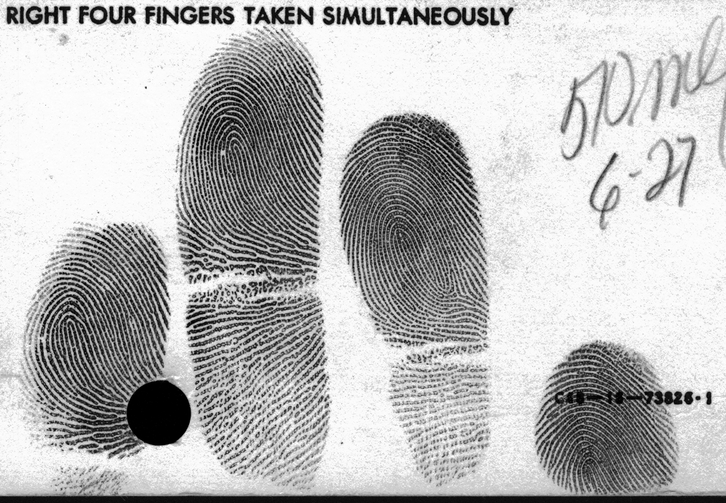
\includegraphics[width=0.49\linewidth]{images/a002-original}\hfill
  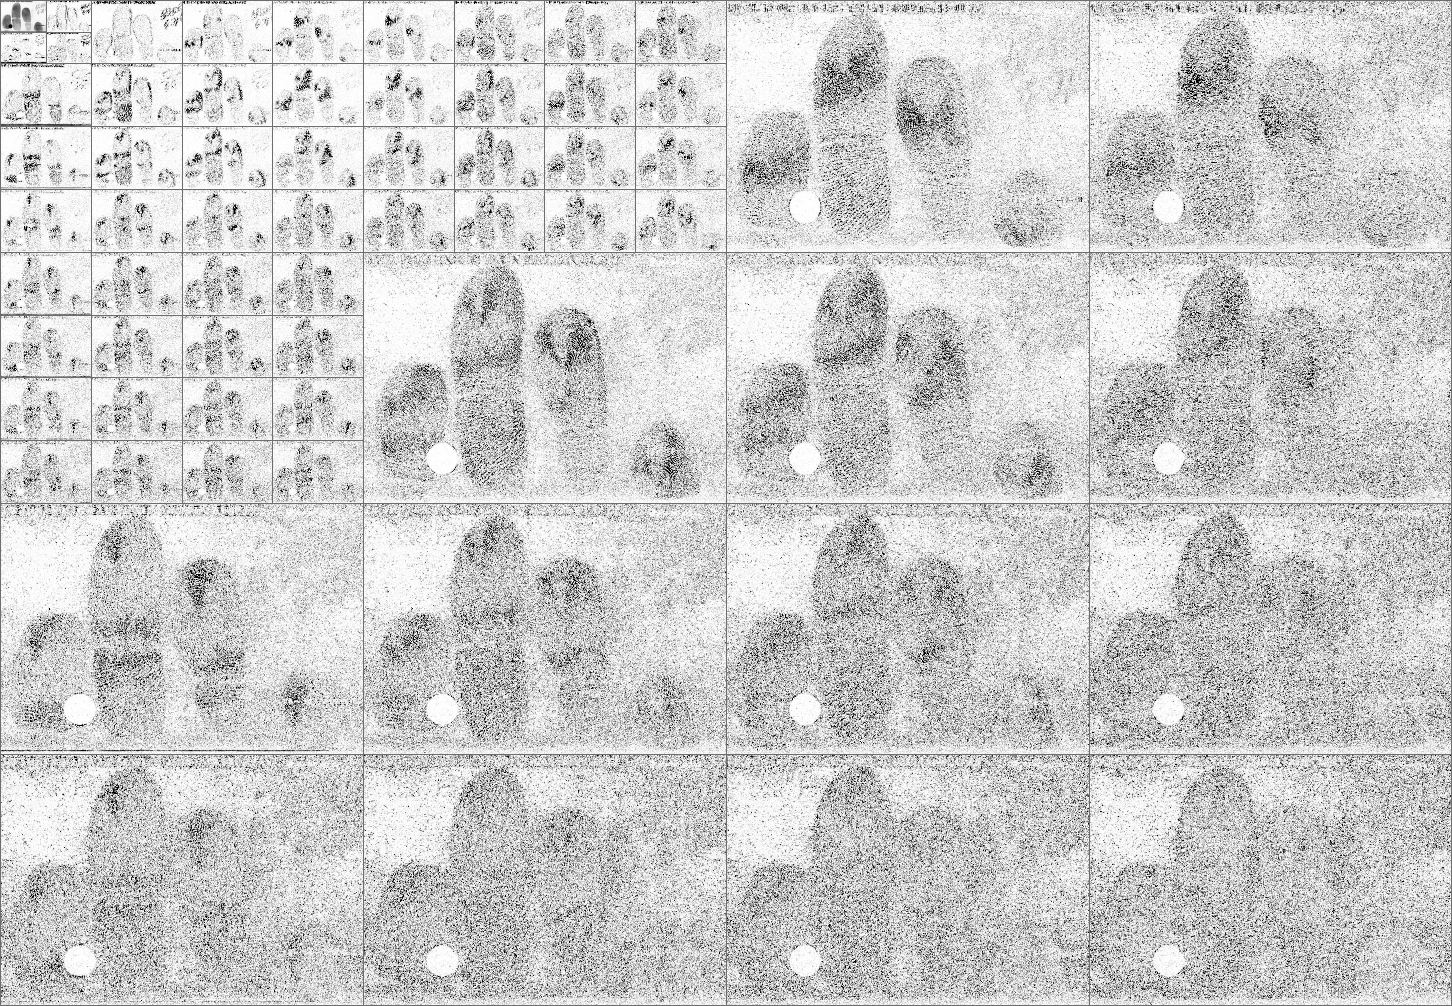
\includegraphics[width=0.49\linewidth]{images/a002-subbands}
  \caption{Image \texttt{a002} of the NIST compliance set ($1452 \times 1006$, a slap of four
  fingers) and its 64 subbands. Each subband is displayed with its own contrast (darker means
  a larger magnitude), except subband 0, which shows the coefficients themselves.}
  \label{fig:a002subbands}
\end{figure}

\section{Quantization}
\label{sec:quantization}

Quantization is the only lossy step. Each subband gets its own uniform scalar quantizer, and
the art of the encoder lies in choosing the bin widths: fine enough in the subbands that
carry ridge structure, coarse enough elsewhere to reach the target bit rate. The quantizer
itself belongs to Part~1 and is the same for every encoder; how the bin widths are chosen is
the business of Part~3.

\subsection{The dead-zone quantizer}

For subband $k$ with bin width $Q_k > 0$ and zero-bin width $Z_k$, a coefficient $a$ is mapped
to the integer index (Annex A.3)
\begin{equation}
  p = \begin{cases}
    \floor{(a - Z_k/2)/Q_k} + 1, & a > Z_k/2,\\
    0, & -Z_k/2 \le a \le Z_k/2,\\
    \ceil{(a + Z_k/2)/Q_k} - 1, & a < -Z_k/2,
  \end{cases}
  \label{eq:quantize}
\end{equation}
and the decoder maps it back to
\begin{equation}
  \hat a = \begin{cases}
    (p - C)\,Q_k + Z_k/2, & p > 0,\\
    0, & p = 0,\\
    (p + C)\,Q_k - Z_k/2, & p < 0.
  \end{cases}
  \label{eq:dequantize}
\end{equation}
Figure~\ref{fig:quantizer} shows the bins. The zero bin is wider than the others
($Z_k = 1.2\,Q_k$ in encoder number two), a \emph{dead zone} that sends more of the many small
coefficients to zero; zeros are what the entropy coder compresses best, since it codes runs of
them with a single symbol. The parameter $C$ sets where in its bin a nonzero index is
reconstructed. Encoder number two uses $C = 0.44$, which puts $\hat a$ at $0.56\,Q_k$ from the
inner edge of the bin, slightly beyond its middle. A bin width $Q_k = 0$ means that subband $k$
is not transmitted at all: the decoder sets all its coefficients to zero.

\begin{figure}[ht]
  \centering
  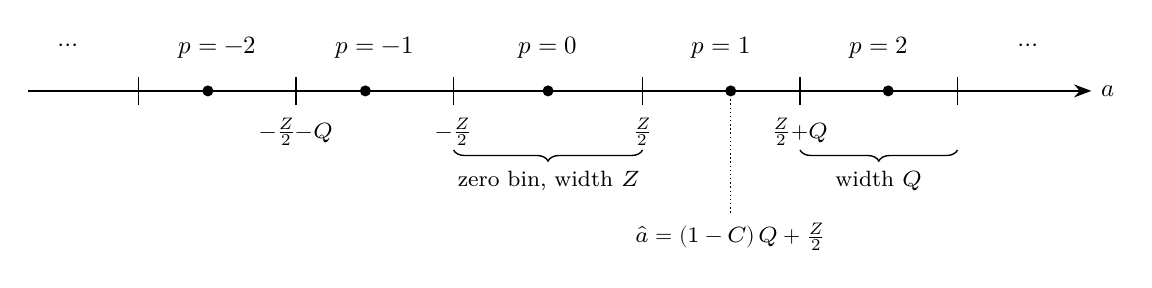
\begin{tikzpicture}[x=1cm,y=1cm,font=\small]
  % Z = 2.4, Q = 2 (Z = 1.2 Q); C = 0.44
  \def\Zh{1.2}\def\Q{2}\def\C{0.44}
  \draw[->] (-6.6,0) -- (6.9,0) node[right] {$a$};
  % bin edges
  \foreach \s in {-1,1} {
    \foreach \i in {0,1,2} {
      \pgfmathsetmacro{\e}{\s*(\Zh+\i*\Q)}
      \draw (\e,-0.18) -- (\e,0.18);
    }
  }
  \node[below=1mm,font=\footnotesize] at (\Zh,-0.12) {$\tfrac{Z}{2}$};
  \node[below=1mm,font=\footnotesize] at (-\Zh,-0.12) {$-\tfrac{Z}{2}$};
  \node[below=1mm,font=\footnotesize] at (\Zh+\Q,-0.12) {$\tfrac{Z}{2}{+}Q$};
  \node[below=1mm,font=\footnotesize] at (-\Zh-\Q,-0.12) {$-\tfrac{Z}{2}{-}Q$};
  % indices
  \node at (0,0.55) {$p=0$};
  \foreach \i in {1,2} {
    \pgfmathsetmacro{\c}{\Zh+(\i-0.5)*\Q}
    \node at (\c,0.55) {$p=\i$};
    \node at (-\c,0.55) {$p=-\i$};
  }
  \node at (6.1,0.55) {$\cdots$};
  \node at (-6.1,0.55) {$\cdots$};
  % reconstruction points (p - C) Q + Z/2
  \foreach \i in {1,2} {
    \pgfmathsetmacro{\r}{(\i-\C)*\Q+\Zh}
    \fill (\r,0) circle (0.07);
    \fill (-\r,0) circle (0.07);
  }
  \fill (0,0) circle (0.07);
  % braces
  \draw[decorate,decoration={brace,amplitude=4pt,mirror}] (-\Zh,-0.75) -- (\Zh,-0.75)
    node[midway,below=4pt,font=\footnotesize] {zero bin, width $Z$};
  \draw[decorate,decoration={brace,amplitude=4pt,mirror}] (\Zh+\Q,-0.75) -- (\Zh+2*\Q,-0.75)
    node[midway,below=4pt,font=\footnotesize] {width $Q$};
  \pgfmathsetmacro{\ra}{(1-\C)*\Q+\Zh}
  \draw[densely dotted] (\ra,0) -- (\ra,-1.55) node[below,font=\footnotesize] {$\hat a = (1-C)\,Q + \tfrac{Z}{2}$};
\end{tikzpicture}

  \caption{The dead-zone scalar quantizer with $Z = 1.2\,Q$. Dots mark the reconstruction
  values for $C = 0.44$.}
  \label{fig:quantizer}
\end{figure}

\subsection{Subband variances}
\label{sec:variance}

Encoder number two chooses the bin widths from the variance of each subband. Fingerprints
rarely fill the scanned area, and the background around them would make the variances
unrepresentative, so the variance is normally estimated on a central window of each subband
(Part 3, Section 3.1). For a subband of $X_k \times Y_k$ coefficients the window has
\begin{equation}
  X'_k = \floor{3X_k/4} \text{ columns starting at } \floor{X_k/8}, \qquad
  Y'_k = \floor{7Y_k/16} \text{ rows starting at } \floor{9Y_k/32},
  \label{eq:window}
\end{equation}
as in Figure~\ref{fig:window}: up to rounding, the window is centred and covers three quarters
of the width and seven sixteenths of the height. The variance is the unbiased estimate over the
window,
\begin{equation}
  \sigma_k^2 = \frac{1}{X'_kY'_k - 1}\sum_{m,n \in \text{window}} \bigl(a_k(m,n) - \mu_k\bigr)^2,
  \label{eq:variance}
\end{equation}
where $\mu_k$ is the mean over the window.

\begin{figure}[ht]
  \centering
  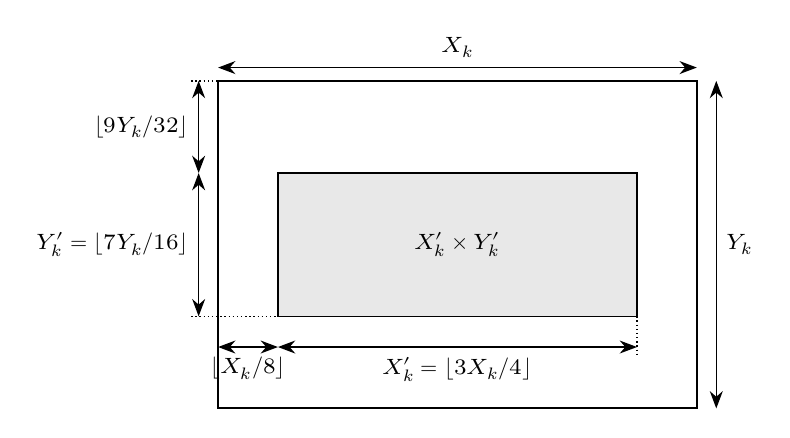
\begin{tikzpicture}[x=0.19cm,y=-0.13cm,font=\footnotesize]
  % subband of 32 x 32 units; window x0 = X/8 = 4, width 3X/4 = 24; y0 = 9Y/32 = 9, height 7Y/16 = 14
  \draw[line width=0.7pt] (0,0) rectangle (32,32);
  \fill[gray!18] (4,9) rectangle (28,23);
  \draw (4,9) rectangle (28,23);
  \node at (16,16) {$X'_k \times Y'_k$};
  \draw[<->] (0,-1.3) -- node[above] {$X_k$} (32,-1.3);
  \draw[<->] (33.3,0) -- node[right] {$Y_k$} (33.3,32);
  \draw[<->] (0,26) -- node[below] {$\floor{X_k/8}$} (4,26);
  \draw[<->] (4,26) -- node[below] {$X'_k = \floor{3X_k/4}$} (28,26);
  \draw[<->] (-1.3,0) -- node[left] {$\floor{9Y_k/32}$} (-1.3,9);
  \draw[<->] (-1.3,9) -- node[left] {$Y'_k = \floor{7Y_k/16}$} (-1.3,23);
  \draw[densely dotted] (0,26) -- (0,32) (28,23) -- (28,27);
  \draw[densely dotted] (-1.8,0) -- (0,0) (-1.8,23) -- (4,23);
\end{tikzpicture}

  \caption{The window used to estimate the variance of a subband.}
  \label{fig:window}
\end{figure}

Version~3.1 of the specification added a safeguard, and this is the whole difference between
encoder number one and encoder number two. Live-scan devices with 3-inch platens capture two
thumbs side by side, and when the thumbs rest near the bottom edge they fall outside the
window. The window variances then describe the background rather than the prints, the bin
widths are chosen badly, and in extreme cases every print is lost from the decoded image
\cite{nistnotice}. The fix tests the
four lowest-frequency subbands: if
\begin{equation}
  \sigma_0^2 + \sigma_1^2 + \sigma_2^2 + \sigma_3^2 > 20\,000
\end{equation}
with the window estimates, the window is used for every subband; otherwise every variance is
recomputed over the whole subband ($X'_k = X_k$, $Y'_k = Y_k$, starting at the corner). NIST
reports that about 12\% of two-thumb images switch to the full region, and fewer than 0.5\% of
other impressions do. In the NIST compliance set, 7 of the 40 images do.

\subsection{Bin widths}
\label{sec:binwidths}

The bin widths come from a classical bit-allocation argument \cite{bradley1993}. Assume that the
coefficients of subband $k$ lie in an interval of $2\gamma$ standard deviations,
$[\mu_k - \gamma\sigma_k, \mu_k + \gamma\sigma_k]$ with \emph{loading factor} $\gamma = 2.5$.
(Outliers do no harm, because the entropy coder handles them with escape codes.) A quantizer
with bin width $Q_k$ then has $L_k = 2\gamma\sigma_k/Q_k$ bins and spends
$r_k = \log_2 L_k$ bits per coefficient. Subband $k$ has $XY/m_k$ coefficients, so the average
rate over the image is
\begin{equation}
  r = \sum_{k \in K} \frac{r_k}{m_k} = \sum_{k \in K} \frac{1}{m_k}\log_2\frac{2\gamma\sigma_k}{Q_k}
  \quad\text{bits per pixel},
  \label{eq:rate}
\end{equation}
where $K$ is the set of subbands that receive bits. This is the constraint; the remaining
freedom is the \emph{relative} widths. Encoder number two fixes them as
\begin{equation}
  Q_k = Q'_k / q, \qquad
  Q'_k = \begin{cases}
    1, & 0 \le k \le 3,\\
    \dfrac{10}{A_k \ln \sigma_k^2}, & 4 \le k \le 59,\\
    0, & 60 \le k \le 63 \text{ or } \sigma_k^2 < 1.01,
  \end{cases}
  \qquad Z_k = 1.2\,Q_k,
  \label{eq:relwidths}
\end{equation}
with weights $A_k = 1.32$ for $k \in \{52, 56\}$, $1.08$ for $k \in \{53, 55, 58, 59\}$,
$1.42$ for $k \in \{54, 57\}$, and $1$ otherwise. The logarithm makes high-variance subbands
(the ones with ridge structure) get finer bins, the weights fine-tune the quarter-size
subbands, and subbands with almost no variance are dropped. The single constant $q$ scales all
widths together. Substituting $Q_k = Q'_k/q$ into Equation~\eqref{eq:rate} and writing
$S = \sum_{k\in K} 1/m_k$ for the fraction of coefficients that receive bits gives
$r = S\log_2(2\gamma q) + \sum_{k\in K} m_k^{-1}\log_2(\sigma_k/Q'_k)$, and solving for $q$,
\begin{equation}
  q = \frac{2^{r/S - 1}}{\gamma}\,
      \Biggl[\,\prod_{k\in K}\Bigl(\frac{\sigma_k}{Q'_k}\Bigr)^{1/m_k}\Biggr]^{-1/S}.
  \label{eq:q}
\end{equation}

One complication remains. If a subband's bin turns out wider than its whole range,
$Q_k \ge 2\gamma\sigma_k$, the model gives it a negative rate $r_k$, which is meaningless and
would let the other subbands overspend. Such subbands are removed from $K$ and $q$ is
recomputed, until no subband is left with a nonpositive rate (Algorithm~\ref{alg:binwidths}).
The removed subbands are still quantized with the final widths: they are expected to quantize
almost entirely to zero, but the few coefficients that survive are kept.

\begin{algorithm}[ht]
  \caption{Bin widths of encoder number two (Part 3, Section 3.2).}
  \label{alg:binwidths}
  \begin{algorithmic}[1]
    \Require subband variances $\sigma_k^2$ ($k = 0..59$); target rate $r$ in bits per pixel; $\gamma = 2.5$
    \Ensure bin widths $Q_k$ and $Z_k$ for $k = 0..63$
    \State compute $Q'_k$ by Eq.~\eqref{eq:relwidths}
    \State $K_0 \gets \{k \le 59 : \sigma_k^2 \ge 1.01\}$;\ $K \gets K_0$
    \Loop
      \State $S \gets \sum_{k\in K} 1/m_k$
      \State $q \gets \gamma^{-1}\, 2^{r/S - 1} \bigl[\prod_{k\in K} (\sigma_k/Q'_k)^{1/m_k}\bigr]^{-1/S}$
      \State $\Xi \gets \{k \in K : Q'_k/q \ge 2\gamma\sigma_k\}$ \Comment{nonpositive rates}
      \If{$\Xi = \emptyset$} \textbf{break} \EndIf
      \State $K \gets K \setminus \Xi$
    \EndLoop
    \For{$k \gets 0$ \textbf{to} $63$}
      \State $Q_k \gets Q'_k/q$ \textbf{if} $k \in K_0$ \textbf{else} $0$;\quad $Z_k \gets 1.2\,Q_k$
    \EndFor
  \end{algorithmic}
\end{algorithm}

The rate $r$ is only a target, since the model ignores how the entropy coder actually behaves.
On the 40 images of the NIST compliance set, the NIST encoder asked for $r = 0.75$ produced
files of 0.53 bits per pixel on average (from 0.19 to 0.75, counting the whole file), and
asked for $r = 2.25$, files of 1.66 bits per pixel (from 0.35 to 2.31).

\section{Entropy coding}
\label{sec:entropy}

After quantization most indices are zero, and the nonzero ones are mostly $\pm1$ or $\pm2$.
WSQ codes them losslessly with a Huffman coder whose alphabet mixes coefficient values with
lengths of zero runs, in the spirit of baseline JPEG (Annex A.4 and Annex C).

\subsection{Blocks}
\label{sec:blocks}

The indices are serialized subband by subband in increasing $k$, row by row within a subband,
skipping subbands with $Q_k = 0$. The sequence is cut into \emph{blocks}, each coded with one
Huffman table. There must be at least three blocks, with breaks between subbands 18 and 19 and
between 51 and 52 (Figure~\ref{fig:subbands}); further subdivision is allowed. The breaks
separate the coarse subbands from the fine ones so that a decoder could show a low-resolution
image after the first block (\emph{progressive transmission}). Encoder number two uses exactly
three blocks, one Huffman table for block~1 (subbands 0--18) and a second, shared table for
blocks 2 and 3 (subbands 19--51 and 52--59). Zero runs may cross subband boundaries within a
block.

\subsection{The symbol alphabet}

Table~\ref{tab:symbols} lists the 254 symbols. Symbols 1 to 100 stand for runs of 1 to 100
zeros, and symbols 107 to 254 for the indices $-73$ to $74$, with symbol $s$ meaning the index
$s - 180$. The index 0 never appears as a value, so symbol 180 is unused: an isolated zero is a
run of length one. Anything outside these ranges is coded with an escape symbol followed by the
raw value in 8 or 16 bits, most significant bit first. Indices are signed, but the escape
carries the magnitude and the symbol carries the sign. Algorithm~\ref{alg:tokenize} turns a
block into symbols the way the NIST encoder does, which also fixes the choices the
specification leaves open (for example, a run of 300 zeros becomes one 16-bit escape rather
than several shorter runs).

\begin{table}[ht]
  \centering\small
  \begin{tabular}{@{}rl@{}}
    \toprule
    symbol $s$ & meaning\\
    \midrule
    1--100 & a run of $s$ zeros\\
    101 & escape: positive index, 8-bit magnitude follows\\
    102 & escape: negative index, 8-bit magnitude follows\\
    103 & escape: positive index, 16-bit magnitude follows\\
    104 & escape: negative index, 16-bit magnitude follows\\
    105 & escape: run of zeros, 8-bit length follows\\
    106 & escape: run of zeros, 16-bit length follows\\
    107--254 & the index $s - 180$, from $-73$ to $74$ (symbol 180 is never used)\\
    \bottomrule
  \end{tabular}
  \caption{Huffman input symbols (Table A.2 of the specification).}
  \label{tab:symbols}
\end{table}

\begin{algorithm}[ht]
  \caption{Turning a block of indices into symbols (as in the NIST encoder).}
  \label{alg:tokenize}
  \begin{algorithmic}[1]
    \Require indices $p_1, \dots, p_N$ of one block
    \Ensure symbols, each possibly followed by an extra field of $b$ raw bits
    \Procedure{EmitRun}{$n$}
      \If{$n \le 100$} emit symbol $n$
      \ElsIf{$n \le 255$} emit $105$ and $n$ in 8 bits
      \Else\ emit $106$ and $n$ in 16 bits
      \EndIf
    \EndProcedure
    \State $n \gets 0$
    \For{$i \gets 1$ \textbf{to} $N$}
      \If{$p_i = 0$}
        \State $n \gets n + 1$
        \If{$n = 65535$} \Call{EmitRun}{$n$};\ $n \gets 0$ \EndIf
      \Else
        \If{$n > 0$} \Call{EmitRun}{$n$};\ $n \gets 0$ \EndIf
        \If{$-73 \le p_i \le 74$} emit symbol $p_i + 180$
        \ElsIf{$0 < p_i \le 255$} emit $101$ and $p_i$ in 8 bits
        \ElsIf{$p_i > 255$} emit $103$ and $p_i$ in 16 bits
        \ElsIf{$-255 \le p_i < 0$} emit $102$ and $-p_i$ in 8 bits
        \Else\ emit $104$ and $-p_i$ in 16 bits
        \EndIf
      \EndIf
    \EndFor
    \If{$n > 0$} \Call{EmitRun}{$n$} \EndIf
  \end{algorithmic}
\end{algorithm}

\subsection{Huffman tables}

A Huffman table is transmitted in the compact form of JPEG: a list $\mathrm{BITS}$ of 16
counts, $\mathrm{BITS}(\ell)$ being the number of codes of length $\ell$ bits, followed by the
list $\mathrm{HUFFVAL}$ of the symbols, sorted by code length (Annex C). The codes themselves
are not transmitted: both sides derive them by the \emph{canonical} rule. Codes of the same
length are consecutive binary numbers, the first code of each length follows the last code of
the previous length, and each step to a longer length appends a zero
(Algorithm~\ref{alg:codes}, which merges Figures C.1 and C.2 of the specification).

Figure~\ref{fig:hufftree} shows an example with $\mathrm{BITS} = (0, 2, 3, 1, 0, \dots)$ and
$\mathrm{HUFFVAL} = (1, 181, 179, 2, 182, 3)$. The specification requires that the code made
only of 1-bits be left unused at every length, as JPEG does. A decoder that looks for markers
can then never mistake the 1-bit padding at the end of a segment for a code.

\begin{figure}[ht]
  \centering
  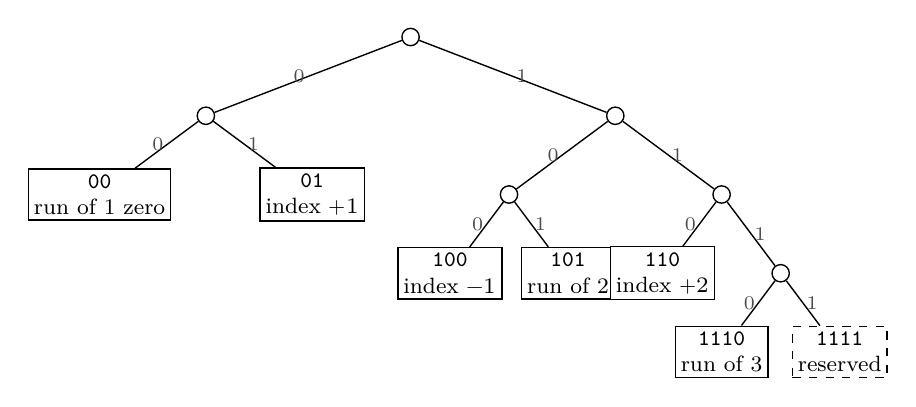
\begin{tikzpicture}[level distance=10mm,font=\footnotesize,
    inner/.style={circle,draw,fill=white,inner sep=0pt,minimum size=2.2mm},
    leaf/.style={draw,align=center,inner sep=2pt,fill=white},
    level 1/.style={sibling distance=52mm},
    level 2/.style={sibling distance=27mm},
    level 3/.style={sibling distance=15mm},
    edge from parent/.style={draw},
    bit/.style={font=\scriptsize,text=black!70,inner sep=1pt}]
  \node[inner] {}
    child {node[inner] {}
      child {node[leaf] {\texttt{00}\\run of 1 zero} edge from parent node[bit,left] {0}}
      child {node[leaf] {\texttt{01}\\index $+1$} edge from parent node[bit,right] {1}}
      edge from parent node[bit,left] {0}}
    child {node[inner] {}
      child {node[inner] {}
        child {node[leaf] {\texttt{100}\\index $-1$} edge from parent node[bit,left] {0}}
        child {node[leaf] {\texttt{101}\\run of 2} edge from parent node[bit,right] {1}}
        edge from parent node[bit,left] {0}}
      child {node[inner] {}
        child {node[leaf] {\texttt{110}\\index $+2$} edge from parent node[bit,left] {0}}
        child {node[inner] {}
          child {node[leaf] {\texttt{1110}\\run of 3} edge from parent node[bit,left] {0}}
          child {node[leaf,dashed] {\texttt{1111}\\reserved} edge from parent node[bit,right] {1}}
          edge from parent node[bit,right] {1}}
        edge from parent node[bit,right] {1}}
      edge from parent node[bit,right] {1}};
\end{tikzpicture}

  \caption{Canonical code tree for $\mathrm{BITS} = (0,2,3,1)$ and
  $\mathrm{HUFFVAL} = (1, 181, 179, 2, 182, 3)$. The all-ones word \texttt{1111} is reserved.}
  \label{fig:hufftree}
\end{figure}

\begin{algorithm}[ht]
  \caption{Canonical codes and decoding tables from BITS and HUFFVAL.}
  \label{alg:codes}
  \begin{algorithmic}[1]
    \Require $\mathrm{BITS}(1..16)$, $\mathrm{HUFFVAL}(0..n-1)$ with $n = \sum_\ell \mathrm{BITS}(\ell)$
    \Ensure $\mathrm{code}(i)$ and $\mathrm{size}(i)$ for symbol $\mathrm{HUFFVAL}(i)$; tables $\mathrm{MINCODE}$, $\mathrm{MAXCODE}$, $\mathrm{VALPTR}$
    \State $c \gets 0$;\ $i \gets 0$
    \For{$\ell \gets 1$ \textbf{to} $16$}
      \If{$\mathrm{BITS}(\ell) = 0$}
        \State $\mathrm{MAXCODE}(\ell) \gets -1$ \Comment{no code of this length}
      \Else
        \State $\mathrm{VALPTR}(\ell) \gets i$;\ $\mathrm{MINCODE}(\ell) \gets c$
        \For{$j \gets 1$ \textbf{to} $\mathrm{BITS}(\ell)$}
          \State $\mathrm{code}(i) \gets c$;\ $\mathrm{size}(i) \gets \ell$;\ $c \gets c + 1$;\ $i \gets i + 1$
        \EndFor
        \State $\mathrm{MAXCODE}(\ell) \gets c - 1$
      \EndIf
      \State $c \gets 2c$ \Comment{one bit longer}
    \EndFor
  \end{algorithmic}
\end{algorithm}

\subsection{Decoding}

Bits are packed into bytes most significant bit first (Annex C.3). A decoder reads one bit at
a time, growing a code until it falls within the range of codes of its length, and then looks
the symbol up (Algorithm~\ref{alg:huffdecode}). The symbol is expanded into indices by reading
Table~\ref{tab:symbols} backwards. Two byte-level rules apply inside an entropy-coded segment
(Annex B.1.1.5): the encoder pads the last byte with 1-bits, and after every \hex{FF} byte it
writes a \hex{00} byte (\emph{byte stuffing}), so that a marker, which is \hex{FF} followed by
a nonzero byte, can never appear by accident. The decoder drops the stuffed zeros and stops at
the first true marker, discarding any incomplete code (the padding).

\begin{algorithm}[ht]
  \caption{Decoding the indices of one block.}
  \label{alg:huffdecode}
  \begin{algorithmic}[1]
    \Require the bits of an entropy-coded segment (stuffing removed); the block's table; the number $N$ of indices still expected
    \Ensure the indices of the block, appended to the output
    \Function{DecodeSymbol}{}
      \State $c \gets$ next bit;\ $\ell \gets 1$
      \While{$c > \mathrm{MAXCODE}(\ell)$}
        \State $c \gets 2c + \text{next bit}$;\ $\ell \gets \ell + 1$
        \If{$\ell > 16$} \textbf{fail}: invalid code \EndIf
      \EndWhile
      \State \Return $\mathrm{HUFFVAL}\bigl(\mathrm{VALPTR}(\ell) + c - \mathrm{MINCODE}(\ell)\bigr)$
    \EndFunction
    \While{fewer than $N$ indices have been produced \textbf{and} bits remain}
      \State $s \gets \Call{DecodeSymbol}{}$ \Comment{stop quietly if the bits run out inside a code}
      \If{$1 \le s \le 100$} output $s$ zeros
      \ElsIf{$s = 101$ \textbf{or} $s = 103$} output the next 8 (16) bits as a positive index
      \ElsIf{$s = 102$ \textbf{or} $s = 104$} output minus the next 8 (16) bits
      \ElsIf{$s = 105$ \textbf{or} $s = 106$} output as many zeros as the next 8 (16) bits say
      \ElsIf{$107 \le s \le 254$ \textbf{and} $s \ne 180$} output $s - 180$
      \Else\ \textbf{fail}: invalid symbol
      \EndIf
    \EndWhile
  \end{algorithmic}
\end{algorithm}

A note of caution: the all-ones rule is not always honoured. Every one of the 86 WSQ files that
NIST distributes for decoder compliance testing contains a Huffman table that assigns an
all-ones code, and the NIST decoder prints a warning for each of them. A decoder should accept
such tables.

\subsection{Designing the tables}

The specification does not say how an encoder builds its tables. Encoder number two builds
them for each image from the symbol counts, using the procedure of Annex K of the JPEG standard
\cite{jpeg}, as the NIST encoder does (Algorithm~\ref{alg:hufftable}). It is ordinary Huffman
code construction with three additions: a dummy symbol with count one is added so that the
longest code, which is all ones, goes to it and is then discarded; codes longer than 16 bits
are shortened by moving leaves up the tree; and ties are broken in favour of the larger symbol
value. The length limit is not a corner case: for 59 of the 160 tables the NIST encoder builds
for its compliance images, plain Huffman construction yields codes of 17 to 20 bits. The tie
rule only matters for reproducing the NIST encoder byte for byte; with it,
Algorithm~\ref{alg:hufftable} reproduces all 160 tables exactly.

\begin{algorithm}[ht]
  \caption{An optimal table from symbol counts (JPEG Annex K.2--K.4).}
  \label{alg:hufftable}
  \begin{algorithmic}[1]
    \Require counts $F(0..255)$ of the symbols of the blocks that share the table
    \Ensure $\mathrm{BITS}(1..16)$ and $\mathrm{HUFFVAL}$
    \State $F(256) \gets 1$ \Comment{dummy symbol: reserves the all-ones code}
    \State $\mathrm{size}(v) \gets 0$ and $\mathrm{next}(v) \gets \bot$ for all $v$ \Comment{each $v$ heads a chain of merged symbols}
    \Loop
      \State $v_1 \gets$ the symbol with the smallest $F > 0$; $v_2 \gets$ the next smallest \Comment{ties: larger $v$ first}
      \If{there is no $v_2$} \textbf{break} \EndIf
      \State $F(v_1) \gets F(v_1) + F(v_2)$;\ $F(v_2) \gets 0$
      \State increment $\mathrm{size}$ of every symbol in the chains of $v_1$ and $v_2$
      \State link the chain of $v_2$ to the end of the chain of $v_1$
    \EndLoop
    \State $\mathrm{B}(\ell) \gets |\{v : \mathrm{size}(v) = \ell\}|$ for $\ell = 1..32$
    \For{$\ell \gets 32$ \textbf{down to} $17$} \Comment{limit lengths to 16 bits}
      \While{$\mathrm{B}(\ell) > 0$}
        \State $j \gets \ell - 2$; \textbf{while} $\mathrm{B}(j) = 0$: $j \gets j - 1$
        \State $\mathrm{B}(\ell) \gets \mathrm{B}(\ell) - 2$;\ $\mathrm{B}(\ell-1) \gets \mathrm{B}(\ell-1) + 1$;\ $\mathrm{B}(j+1) \gets \mathrm{B}(j+1) + 2$;\ $\mathrm{B}(j) \gets \mathrm{B}(j) - 1$
      \EndWhile
    \EndFor
    \State decrement $\mathrm{B}(\ell)$ for the largest $\ell$ with $\mathrm{B}(\ell) > 0$ \Comment{drop the dummy}
    \State $\mathrm{BITS}(\ell) \gets \mathrm{B}(\ell)$ for $\ell = 1..16$
    \State $\mathrm{HUFFVAL} \gets$ symbols $0..255$ with $\mathrm{size} > 0$, by increasing size, then increasing value
  \end{algorithmic}
\end{algorithm}

\section{The file format}
\label{sec:format}

A WSQ file is a sequence of bytes organized like a JPEG file (Annex B). It is made of
\emph{markers}, two-byte codes \hex{FF} followed by a byte other than \hex{00} and \hex{FF};
of \emph{marker segments}, a marker followed by a 16-bit length and a list of parameters; and
of \emph{entropy-coded segments} (ECS), the Huffman-coded data. Multi-byte parameters are
big-endian. The length of a marker segment counts its own two bytes and the parameters, but
not the marker. Any marker may be preceded by any number of \hex{FF} fill bytes.
Table~\ref{tab:markers} lists the markers.

\begin{table}[ht]
  \centering\small
  \begin{tabular}{@{}lll@{}}
    \toprule
    code & name & meaning \\
    \midrule
    \hex{FFA0} & \marker{SOI} & start of image (no segment) \\
    \hex{FFA1} & \marker{EOI} & end of image (no segment) \\
    \hex{FFA2} & \marker{SOF} & start of frame: the frame header \\
    \hex{FFA3} & \marker{SOB} & start of block: the block header \\
    \hex{FFA4} & \marker{DTT} & define transform table (the wavelet filters) \\
    \hex{FFA5} & \marker{DQT} & define quantization table \\
    \hex{FFA6} & \marker{DHT} & define Huffman table(s) \\
    \hex{FFA7} & \marker{DRI} & define restart interval \\
    \hex{FFA8} & \marker{COM} & comment \\
    \hex{FFB0}--\hex{FFB7} & \marker{RST}$_m$ & restart marker, $m = 0..7$ cyclically (no segment) \\
    \bottomrule
  \end{tabular}
  \caption{Marker codes (Table B.1 of the specification).}
  \label{tab:markers}
\end{table}

\subsection{Structure}

A file is \marker{SOI}, one \emph{frame}, \marker{EOI}. The frame is a frame header followed by
one or more blocks; each block is a block header followed by its entropy-coded data. Table and
comment segments may come before the frame header and before any block header. When a table is
defined more than once, the latest definition replaces the earlier ones. Figure~\ref{fig:stream}
shows a file written by the NIST encoder; its segments have lengths 124 (\marker{COM}),
58 (\marker{DTT}), 389 (\marker{DQT}), 17 (\marker{SOF}), 193 and 149 (the two \marker{DHT}) and
3 (each \marker{SOB}).

\begin{figure}[ht]
  \centering
  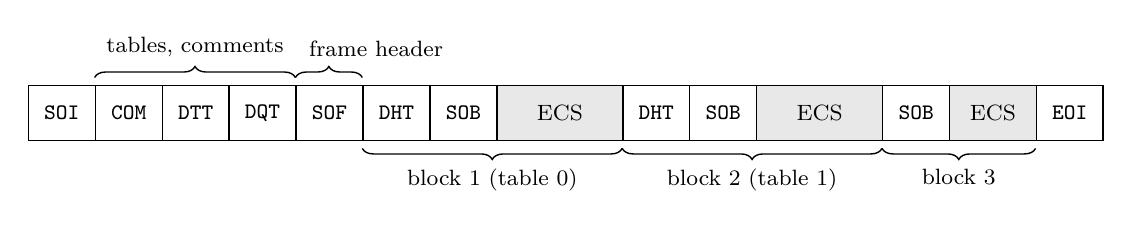
\begin{tikzpicture}[x=1cm,y=1cm,font=\footnotesize,
    seg/.style={draw,minimum height=7mm,inner sep=1pt,anchor=west},
    ecs/.style={seg,fill=gray!18}]
  \def\row#1{%
    \foreach \name/\w/\st [remember=\x as \lastx (initially 0)] in {#1} {
      \pgfmathsetmacro{\x}{\lastx+\w}
      \node[\st,minimum width=\w cm] at (\lastx,0) {\name};
    }}
  \begin{scope}
    \row{\marker{SOI}/0.85/seg, \marker{COM}/0.85/seg, \marker{DTT}/0.85/seg, \marker{DQT}/0.85/seg,
         \marker{SOF}/0.85/seg, \marker{DHT}/0.85/seg, \marker{SOB}/0.85/seg, ECS/1.6/ecs,
         \marker{DHT}/0.85/seg, \marker{SOB}/0.85/seg, ECS/1.6/ecs,
         \marker{SOB}/0.85/seg, ECS/1.1/ecs, \marker{EOI}/0.85/seg}
  \end{scope}
  \draw[decorate,decoration={brace,amplitude=4pt}] (0.85,0.45) -- (3.4,0.45)
    node[midway,above=4pt] {tables, comments};
  \draw[decorate,decoration={brace,amplitude=4pt}] (3.4,0.45) -- (4.25,0.45)
    node[midway,above=4pt,xshift=6mm] {frame header};
  \draw[decorate,decoration={brace,amplitude=4pt,mirror}] (4.25,-0.45) -- (7.55,-0.45)
    node[midway,below=4pt] {block 1 (table 0)};
  \draw[decorate,decoration={brace,amplitude=4pt,mirror}] (7.55,-0.45) -- (10.85,-0.45)
    node[midway,below=4pt] {block 2 (table 1)};
  \draw[decorate,decoration={brace,amplitude=4pt,mirror}] (10.85,-0.45) -- (12.8,-0.45)
    node[midway,below=4pt] {block 3};
\end{tikzpicture}

  \caption{Layout of a file written by the NIST encoder. Shaded boxes are entropy-coded data.}
  \label{fig:stream}
\end{figure}

The specification also defines two \emph{abbreviated formats}: compressed image data with some
or all tables omitted, to be decoded with tables installed earlier, and a file with tables but
no frame, used only to install tables (\marker{SOI}, tables, \marker{EOI}). In the ordinary
\emph{interchange format} every table needed to decode the image is present.

\subsection{Scaled integers}
\label{sec:scaled}

Real-valued parameters (the normalization constants, the filter taps, the bin widths) are
stored as a pair: an 8-bit exponent $E$ and an unsigned integer $V$ of 16 or 32 bits, meaning
$V/10^E$. The specification does not say how to choose $E$. The NIST encoder takes the largest
$E$ for which the rounded $V$ still fits, which keeps four to five significant digits for 16-bit
values and nine to ten for 32-bit ones: starting from the value, it multiplies by 10 until the
result reaches the largest unsigned value ($65535$ or $2^{32}-1$), steps back once, and rounds.
Zero is stored as $E = 0$, $V = 0$. Signs, where needed, travel in a separate byte.

\subsection{Segments}

Tables~\ref{tab:sof} to~\ref{tab:dht} give the layout of each segment, field by field, with
the sizes in bits and the values the NIST encoder writes.

\begin{table}[ht]
  \centering\small
  \begin{tabular}{@{}llp{9.3cm}@{}}
    \toprule
    field & bits & meaning \\
    \midrule
    $L_f$ & 16 & segment length, 17 \\
    $A$ & 8 & scanner black calibration value (0) \\
    $B$ & 8 & scanner white calibration value (255) \\
    $Y$ & 16 & number of lines (image height) \\
    $X$ & 16 & samples per line (image width) \\
    $E_m$, $M$ & 8, 16 & normalization shift $M$ as a scaled integer \\
    $E_r$, $R$ & 8, 16 & normalization scale $R$ as a scaled integer \\
    $E_v$ & 8 & encoder number: 2 for encoder number two (the value version 3.1 introduced) \\
    $S_f$ & 16 & software implementation number (0) \\
    \bottomrule
  \end{tabular}
  \caption{Frame header (\marker{SOF}, Figure B.3).}
  \label{tab:sof}
\end{table}

\begin{table}[ht]
  \centering\small
  \begin{tabular}{@{}llp{9.3cm}@{}}
    \toprule
    field & bits & meaning \\
    \midrule
    \multicolumn{3}{@{}l}{\textit{Block header} (\marker{SOB}, Figure B.4)}\\
    $L_s$ & 16 & segment length, 3 \\
    $T_d$ & 8 & Huffman table used by this block, 0 to 7 \\
    \midrule
    \multicolumn{3}{@{}l}{\textit{Transform table} (\marker{DTT}, Figure B.6)}\\
    $L_t$ & 16 & segment length (58 for the 9/7 bank) \\
    $L_0$, $L_1$ & 8, 8 & lengths of $h_0$ and $h_1$ \\
    $S_n$, $E_x$, $H$ & 8, 8, 32 & for each transmitted tap, first of $h_0$ then of $h_1$, starting at the
      centre: sign (nonzero means negative), exponent and magnitude; $\ceil{L_i/2}$ taps per filter \\
    \midrule
    \multicolumn{3}{@{}l}{\textit{Quantization table} (\marker{DQT}, Figure B.7)}\\
    $L_q$ & 16 & segment length, 389 \\
    $E_c$, $C$ & 8, 16 & bin centre parameter $C$ (encoder number two: $E_c = 2$, $C = 44$) \\
    $E_q$, $Q_k$, $E_z$, $Z_k$ & 8, 16, 8, 16 & for $k = 0..63$: bin width and zero-bin width \\
    \midrule
    \multicolumn{3}{@{}l}{\textit{Restart interval} (\marker{DRI}, Figure B.9)}\\
    $L_r$ & 16 & segment length, 4 \\
    $R_i$ & 16 & coefficients per restart interval; 0 disables restarts \\
    \midrule
    \multicolumn{3}{@{}l}{\textit{Comment} (\marker{COM}, Figure B.10)}\\
    $L_c$ & 16 & segment length \\
    $C_m$ & $8(L_c-2)$ & comment bytes, interpreted by the application \\
    \bottomrule
  \end{tabular}
  \caption{Block header and table segments.}
  \label{tab:segments}
\end{table}

\begin{table}[ht]
  \centering\small
  \begin{tabular}{@{}llp{9.3cm}@{}}
    \toprule
    field & bits & meaning \\
    \midrule
    $L_h$ & 16 & segment length \\
    \multicolumn{3}{@{}l}{\textit{then, for each table, until the segment ends:}}\\
    $T_h$ & 8 & table number, 0 to 7 \\
    $L_1,\dots,L_{16}$ & $16\times 8$ & $\mathrm{BITS}$: number of codes of each length \\
    $V_{i,j}$ & $8\sum_i L_i$ & $\mathrm{HUFFVAL}$: the symbols, by increasing code length \\
    \bottomrule
  \end{tabular}
  \caption{Huffman table segment (\marker{DHT}, Figure B.8). One segment may define several
  tables; the NIST encoder writes one segment per table.}
  \label{tab:dht}
\end{table}

\subsection{Restart intervals}

If a \marker{DRI} segment sets a nonzero interval $R_i$, the encoder ends an entropy-coded
segment after every $R_i$ coefficients and writes a restart marker, cycling through
\marker{RST}$_0$ to \marker{RST}$_7$; the decoder can then resynchronize after an error. The
bit buffer is padded and flushed at each restart. Restarts are optional and the NIST encoder
never uses them.

\subsection{Resolution and the NISTCOM comment}

The frame header carries no resolution. In ANSI/NIST-ITL transactions the resolution is a field
of the record that contains the WSQ data. Standalone files written by the NIST tools carry it in
a comment segment that begins with the text \texttt{NIST\_COM} and continues with
\texttt{KEY value} lines, for example
\begin{center}\small
\texttt{NIST\_COM 9 \quad PIX\_WIDTH 1452 \quad PIX\_HEIGHT 1006 \quad PIX\_DEPTH 8 \quad PPI 500}\\
\texttt{LOSSY 1 \quad COLORSPACE GRAY \quad COMPRESSION WSQ \quad WSQ\_BITRATE 0.750000}
\end{center}
This \emph{NISTCOM} convention comes from NBIS, not from the WSQ specification, but readers
commonly rely on it.

\subsection{Parsing}

Algorithm~\ref{alg:parse} reads a file. Each table segment updates the decoder state; each block
header starts an entropy-coded segment, which ends at the first marker that is not a restart
marker.

\begin{algorithm}[ht]
  \caption{Reading a WSQ file.}
  \label{alg:parse}
  \begin{algorithmic}[1]
    \Require the bytes of a file
    \Ensure frame parameters, tables, and a list of blocks (table number, entropy-coded bytes)
    \Function{ReadMarker}{}
      \State require byte \hex{FF}; skip further \hex{FF} bytes; \Return \hex{FF00} $+$ next byte
    \EndFunction
    \State require \Call{ReadMarker}{} $=$ \marker{SOI}
    \Loop
      \State $m \gets \Call{ReadMarker}{}$
      \If{$m = \marker{EOI}$} \textbf{break} \EndIf
      \State $L \gets$ 16-bit length;\ the segment ends $L$ bytes after the length field starts
      \If{$m = \marker{DTT}$} read $L_0$, $L_1$ and the taps; expand $h_0, h_1$; derive $f_0, f_1$ by Eq.~\eqref{eq:antialias}
      \ElsIf{$m = \marker{DQT}$} read $C$ and $Q_k$, $Z_k$ for $k = 0..63$
      \ElsIf{$m = \marker{DHT}$} read tables until the segment ends; build them with Algorithm~\ref{alg:codes}
      \ElsIf{$m = \marker{DRI}$} read $R_i$
      \ElsIf{$m = \marker{COM}$} keep the bytes (look for \texttt{NIST\_COM} and \texttt{PPI})
      \ElsIf{$m = \marker{SOF}$} read $Y$, $X$, $M$, $R$, $E_v$
      \ElsIf{$m = \marker{SOB}$}
        \State read $T_d$; collect bytes up to the next marker other than \marker{RST}$_m$,
               replacing each \hex{FF}\,\hex{00} pair by \hex{FF}; record the block
      \Else\ \textbf{fail}: unknown marker
      \EndIf
    \EndLoop
  \end{algorithmic}
\end{algorithm}

\section{Putting it together}
\label{sec:decoding}

With the pieces of the previous sections, the decoder and encoder number two fit in a page each
(Algorithms~\ref{alg:decode} and~\ref{alg:encode}). Both work on a single $X\times Y$ array of
reals in which every subband occupies the rectangle that Algorithm~\ref{alg:tree} assigns to
it, so the wavelet transform runs in place, as in Figure~\ref{fig:a002subbands}.

\begin{algorithm}[ht]
  \caption{The WSQ decoder.}
  \label{alg:decode}
  \begin{algorithmic}[1]
    \Require a WSQ file
    \Ensure an $X \times Y$ image with 8-bit samples
    \State read the file (Algorithm~\ref{alg:parse}): $X$, $Y$, $M$, $R$; filters; $C$, $Q_k$, $Z_k$; Huffman tables; blocks
    \State $(\mathcal{S}, \mathcal{L}) \gets \Call{BuildTree}{X, Y}$ \Comment{Algorithm~\ref{alg:tree}}
    \State $N \gets \sum_{k:\,Q_k > 0} X_kY_k$ \Comment{number of indices to decode}
    \State $p \gets$ empty list
    \For{each block, in order}
      \State append the indices of the block to $p$, using table $T_d$ and expecting $N - |p|$ more \Comment{Algorithm~\ref{alg:huffdecode}}
    \EndFor
    \State \textbf{fail} unless $|p| = N$
    \State $A \gets$ zero array of $Y$ rows and $X$ columns
    \For{$k \gets 0$ \textbf{to} $63$ with $Q_k > 0$}
      \State take the next $X_kY_k$ values of $p$, row by row, as $p_k(m,n)$
      \State $A$ at the rectangle of subband $k$ $\gets \hat a_k(m,n)$ by Eq.~\eqref{eq:dequantize}
    \EndFor
    \State \Call{Inverse}{$A$} \Comment{Algorithm~\ref{alg:transform2d}}
    \State $\hat I(m,n) \gets \min(255, \max(0, \floor{A(m,n)\,R + M + \frac12}))$ \Comment{Eq.~\eqref{eq:denormalize}}
  \end{algorithmic}
\end{algorithm}

\begin{algorithm}[ht]
  \caption{Encoder number two.}
  \label{alg:encode}
  \begin{algorithmic}[1]
    \Require an $X \times Y$ image $I$ with 8-bit samples; target rate $r$ in bits per pixel
    \Ensure a WSQ file
    \State $M, R \gets$ Eq.~\eqref{eq:MR};\ $A(m,n) \gets (I(m,n) - M)/R$
    \State $(\mathcal{S}, \mathcal{L}) \gets \Call{BuildTree}{X, Y}$;\ \Call{Forward}{$A$} \Comment{Algorithms~\ref{alg:tree}, \ref{alg:transform2d}}
    \State $\sigma_k^2 \gets$ window variances for $k = 0..3$ (Eqs.~\eqref{eq:window}, \eqref{eq:variance})
    \State \textbf{if} $\sum_{k=0}^{3}\sigma_k^2 > 20\,000$ \textbf{then} window variances for $k = 4..59$
           \textbf{else} full-subband variances for $k = 0..59$
    \State $Q_k, Z_k \gets$ Algorithm~\ref{alg:binwidths};\ $C \gets 0.44$
    \For{$k \gets 0$ \textbf{to} $59$ with $Q_k > 0$}
      \State $p_k(m,n) \gets$ Eq.~\eqref{eq:quantize} on the coefficients of subband $k$
    \EndFor
    \State symbols of blocks 1, 2, 3 (subbands 0--18, 19--51, 52--59) $\gets$ Algorithm~\ref{alg:tokenize}
    \State table 0 from the counts of block 1, table 1 from the counts of blocks 2 and 3 \Comment{Algorithm~\ref{alg:hufftable}}
    \State write \marker{SOI}; optionally a \marker{COM} with \texttt{NIST\_COM}; \marker{DTT}; \marker{DQT}; \marker{SOF}
    \For{$b \gets 1$ \textbf{to} $3$}
      \State write \marker{DHT} for the block's table if not yet written; write \marker{SOB}
      \State write the codes and extra bits of the block's symbols, MSB first; pad with 1-bits; stuff \hex{00} after each \hex{FF}
    \EndFor
    \State write \marker{EOI}
  \end{algorithmic}
\end{algorithm}

\subsection{What the decoder sees}

Figure~\ref{fig:rates} shows a detail of image \texttt{a002} after compression at three target
rates with the NIST encoder, and Table~\ref{tab:rates} gives the numbers for the whole image.
The usual rate for 500 ppi images is 0.75 bits per pixel; 0.25 is far below anything used in
practice and is included to make the effect of coarse quantization visible.

\begin{figure}[ht]
  \centering
  % Generated by tools/gen_figures.py; do not edit by hand.
\begin{tabular}{@{}c@{\hspace{2mm}}c@{\hspace{2mm}}c@{\hspace{2mm}}c@{}}
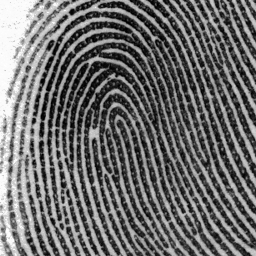
\includegraphics[width=0.24\linewidth]{images/a002-detail-original} & 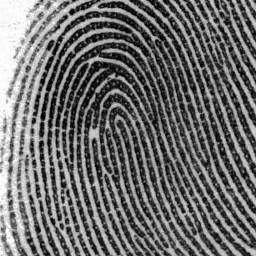
\includegraphics[width=0.24\linewidth]{images/a002-detail-225} & 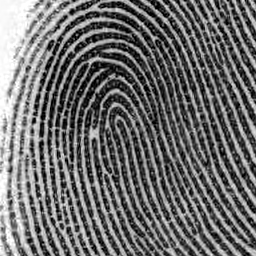
\includegraphics[width=0.24\linewidth]{images/a002-detail-075} & 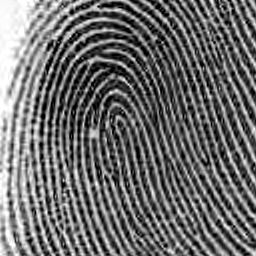
\includegraphics[width=0.24\linewidth]{images/a002-detail-025}\\
original & $r = 2.25$ & $r = 0.75$ & $r = 0.25$\\
\end{tabular}

  \caption{A $256 \times 256$ detail of \texttt{a002}: original and decoded after compression
  with the NIST encoder at three target rates.}
  \label{fig:rates}
\end{figure}

% Generated by tools/gen_figures.py; do not edit by hand.
\begin{table}[ht]
  \centering\small
  \begin{tabular}{@{}rrrrr@{}}
    \toprule
    target $r$ & file size (bytes) & compression ratio & bits per pixel & PSNR (dB)\\
    \midrule
    2.25 & 339\,730 & 4.3\,:\,1 & 1.86 & 34.01\\
    0.75 & 87\,700 & 16.7\,:\,1 & 0.48 & 26.97\\
    0.25 & 28\,784 & 50.7\,:\,1 & 0.16 & 23.29\\
    \bottomrule
  \end{tabular}
  \caption{Image \texttt{a002} (1452$\times$1006, 1\,460\,712 bytes uncompressed) compressed and decoded with NBIS 5.0.0. PSNR is measured over the whole image.}
  \label{tab:rates}
\end{table}


\section{Compliance}
\label{sec:compliance}

Part~2 of the specification defines how an implementation is certified. NIST distributes a set
of test images, the implementer runs them through the encoder and the decoder, and NIST compares
the outputs with those of a reference implementation within the tolerances of Annex AA
(Table~\ref{tab:criteria}). The tolerances accept the small numerical differences between
correct implementations (for instance single against double precision) and nothing more.

\begin{table}[ht]
  \centering\small
  \begin{tabular}{@{}lp{10.6cm}@{}}
    \toprule
    test & requirement \\
    \midrule
    encoder & compressed file size, comments excluded, within 0.4\% of the reference \\
            & every bin width $Q_k$ and zero-bin width $Z_k$ within 0.051\% of the reference \\
            & at least 99.99\% of the quantizer indices equal to the reference, none differing by more than 1 \\
    decoder & at least 99.9\% of the reconstructed pixels equal to the reference, none differing by more than 1 \\
    \bottomrule
  \end{tabular}
  \caption{Compliance criteria (Annex AA).}
  \label{tab:criteria}
\end{table}

The NIST reference data set, version 2.0 \cite{nistcert}, contains
\begin{itemize}
  \item 40 images to encode, in PGM format, between 375 and 1600 pixels wide and 526 and 1500
        pixels high: rolled prints, plain impressions and four-finger slaps, scanned from cards
        or captured live, each to be compressed at 0.75 and at 2.25 bits per pixel;
  \item 86 WSQ files to decode: the same 40 images compressed at each rate, and 6 files that
        use other filter banks (an HS bank with lengths 6 and 10, an HS bank with lengths 10 and 10,
        and a WS bank with lengths 9 and 11);
  \item for two of the files, the quantizer indices of all 60 subbands as text, which allows an
        exact check of the entropy decoder.
\end{itemize}
The reference outputs themselves are not public: certification is done by NIST. The NBIS
software that NIST publishes \cite{nbis}, however, contains the reference encoder and decoder (\texttt{cwsq}
and \texttt{dwsq}), and anyone can apply the criteria of Table~\ref{tab:criteria} against it.

\subsection{How this document was checked}

Every procedure in this document was implemented exactly as written, in double precision and
without optimization, in a short Python program (\texttt{tools/wsqref.py} next to this
document), and compared with NBIS 5.0.0 on the full NIST data set. Table~\ref{tab:checks} shows
the results. The program meets every criterion with a wide margin, and its Huffman tables are
identical to those of NBIS. The remaining differences come from NBIS computing in single
precision.

\begin{table}[ht]
  \centering\small
  \begin{tabular}{@{}lll@{}}
    \toprule
    check & result & criterion \\
    \midrule
    decoded indices of the two reference files & identical in all 60 subbands of both & exact \\
    decoded pixels, 86 files & at least 99.9925\% equal, never more than 1 apart & 99.9\%, 1 \\
    bin widths, 40 images $\times$ 2 rates & within 0.0077\% & 0.051\% \\
    quantizer indices, same 80 cases & at least 99.9955\% equal, never more than 1 apart & 99.99\%, 1 \\
    file size, same 80 cases & within 0.039\% & 0.4\% \\
    Huffman tables built from the NBIS indices & 160 of 160 identical & -- \\
    \bottomrule
  \end{tabular}
  \caption{The algorithms of this document, run as written, against NBIS 5.0.0 on the NIST
  reference data set version 2.0. All 86 decoder cases and all 80 encoder cases pass.}
  \label{tab:checks}
\end{table}

\section{Implementation notes}
\label{sec:implementation}

This section collects the points where an implementation has to go beyond the text of the
specification, or where the NIST reference implementation (NBIS) differs from it. Each item says
whether it was verified while writing this document. The section will grow with the Rust
implementation of the \texttt{wsq-viewer} project, which will add its choices of numerical
precision, its deviations from NBIS, if any, and measured performance.

\begin{description}[leftmargin=0pt]
  \item[Precision.] The specification's \emph{reference} transform is in double precision, while
    NBIS computes in single precision. The double-precision program used for
    Section~\ref{sec:compliance} differs from NBIS by at most one grey level, in fewer than
    0.01\% of the pixels, and by at most one quantizer index (verified).

  \item[The full tree.] NBIS splits the image into 60 subbands and never splits the quadrant of
    subbands 60--63, which encoder number two discards. A decoder that builds all 64 subbands
    produces the same image whenever $Q_{60..63} = 0$, and also decodes the (hypothetical) files
    that use them (verified on the NIST data, where all four are always zero).

  \item[All-ones Huffman codes.] All 86 WSQ files of the NIST decoder test set contain a table
    that assigns an all-ones code, which the specification forbids; NBIS decodes them with a
    warning. A decoder should accept them, and an encoder should never produce them (verified).

  \item[Variance switch.] The specification uses the window when the sum of the four variances
    exceeds 20\,000; NBIS uses it unless the sum is below 20\,000. The two differ only when the sum
    is exactly 20\,000 (from reading the NBIS source).

  \item[Small images.] With the other side large, an image needs at least 49 columns and 81 rows
    (81 pixels on each side for a square) for every variance window to hold two or more
    coefficients. Below that, Equation~\eqref{eq:variance} is undefined for some subband. The
    specification requires compliance only for images of at least 400 pixels on each side and
    says nothing about smaller ones, so an encoder has to choose a behaviour (verified by
    computing the windows for every size).

  \item[Constant images.] A uniform image has $R = 0$ and cannot be normalized by
    Equation~\eqref{eq:normalize}; an encoder has to treat it as a special case.

  \item[Blocks beyond three.] The block headers do not say which subbands a block holds. Since the
    indices are simply concatenated, a decoder decodes each block until its data ends and checks
    at the end that the total matches $\sum_{k:\,Q_k>0} X_kY_k$.

  \item[Untrusted input.] A viewer opens files from anywhere. Image dimensions come from the frame
    header and set the size of every allocation, symbol expansions can produce long runs, and
    tables may be missing, redefined or inconsistent. Every count read from the file has to be
    checked against what remains to be decoded before anything is written.

  \item[Coefficient range.] The escape codes carry at most 16-bit magnitudes, so an index must fit
    in $\pm 65535$. The authors of an independent Rust implementation report that on images with
    almost no detail, such as smooth gradients, encoder number two can produce bins fine enough to
    exceed this range, and that NBIS then wraps the values around \cite{wsqcodec}. This has not
    been verified here yet.
\end{description}

\begin{thebibliography}{99}
\small

\bibitem{wsq31}
Federal Bureau of Investigation, Criminal Justice Information Services Division.
\emph{WSQ Gray-scale Fingerprint Image Compression Specification}, IAFIS-IC-0110 (V3.1).
October 4, 2010.
\url{https://fbibiospecs.fbi.gov/file-repository/wsq_gray-scale_specification_version_3_1_final.pdf}

\bibitem{nistnotice}
National Institute of Standards and Technology.
\emph{WSQ Compression Change in Subband Variance Computation} (announcement), and
C.~Watson, \emph{WSQ Version 3.1} (presentation), March 2011.
\url{https://www.nist.gov/image-group/wsq-bibliography}

\bibitem{nistcert}
National Institute of Standards and Technology.
\emph{WSQ Certification Procedure} and reference image data set version 2.0.
\url{https://www.nist.gov/programs-projects/wsq-certification-procedure}

\bibitem{nbis}
National Institute of Standards and Technology.
\emph{NIST Biometric Image Software (NBIS)}, release 5.0.0, 2015.
\url{https://www.nist.gov/services-resources/software/nist-biometric-image-software-nbis}

\bibitem{brislawn1995}
C.~M.~Brislawn.
Fingerprints go digital.
\emph{Notices of the American Mathematical Society}, 42(11), November 1995.

\bibitem{bradley1994}
J.~N.~Bradley and C.~M.~Brislawn.
The wavelet/scalar quantization compression standard for digital fingerprint images.
In \emph{Proc. IEEE International Symposium on Circuits and Systems (ISCAS)}, 1994.

\bibitem{bradley1993}
J.~N.~Bradley and C.~M.~Brislawn.
Proposed first-generation WSQ bit allocation procedure.
Los Alamos National Laboratory, September 1993.

\bibitem{brislawn1992}
C.~M.~Brislawn.
Classification of symmetric wavelet transforms.
Los Alamos National Laboratory, technical report LA-UR-92-2823, 1992 (revised March 1993).

\bibitem{antonini1992}
M.~Antonini, M.~Barlaud, P.~Mathieu and I.~Daubechies.
Image coding using wavelet transform.
\emph{IEEE Transactions on Image Processing}, 1(2):205--220, 1992.

\bibitem{hopper1992}
T.~Hopper and F.~Preston.
Compression of grey-scale fingerprint images.
In \emph{Proc. Data Compression Conference}, pages 309--318, 1992.

\bibitem{jpeg}
ISO/IEC 10918-1 | ITU-T Recommendation T.81.
\emph{Digital compression and coding of continuous-tone still images: requirements and
guidelines}, 1992. Annex K.

\bibitem{wsqcodec}
\texttt{wsq-codec}, a WSQ decoder and encoder in Rust, version 0.1.1, October 2026.
\url{https://github.com/ybdn/wsq-codec}

\end{thebibliography}


\end{document}
